\documentclass[../main.tex]{subfiles}

\begin{document}
\setcounter{chapter}{1}
\chapter{双端口存储器实验}

\section{实验目的}

\begin{enumerate}

    \item 了解双端口静态存储器 IDT7132 的工作特性及其使用方法;

    \item 了解半导体存储器怎样存储和读取数据;

    \item 了解双端口存储器怎样并行读写;

    \item 熟悉 TEC-8 模型计算机中存储器部分的数据通路.

\end{enumerate}

\section{实验内容}

% 分别在微程序模式和独立模式下进行如下操作:

\begin{enumerate}

    \item 从存储器地址 10H 开始, 通过左端口连续向双端口 RAM 中写入 3 个数: 85H, 60H, 38H. 在写的过程中, 在右端口检测写的数据是否正确;

    \item 从存储器地址 10H 开始, 连续从双端口 RAM 的左端口和右端口同时读出存储器的内容.

\end{enumerate}

\section{实验过程}

\subsection{微程序模式}

\begin{enumerate}

    \item 将操作模式开关设置为 SWC=1, SWB=1, SWA=0, 开启电源, 按一次 QD 按钮, 进入双端口存储器实验.

    \item 在数据开关上设置地址 10H. 通过数据开关依次写入 85H, 60H, 38H, 观察相关变化. (如图\ref{fig:2.1}所示.)

          \begin{figure}[p]
              \centering
              \subfigure[数据85H]{
                  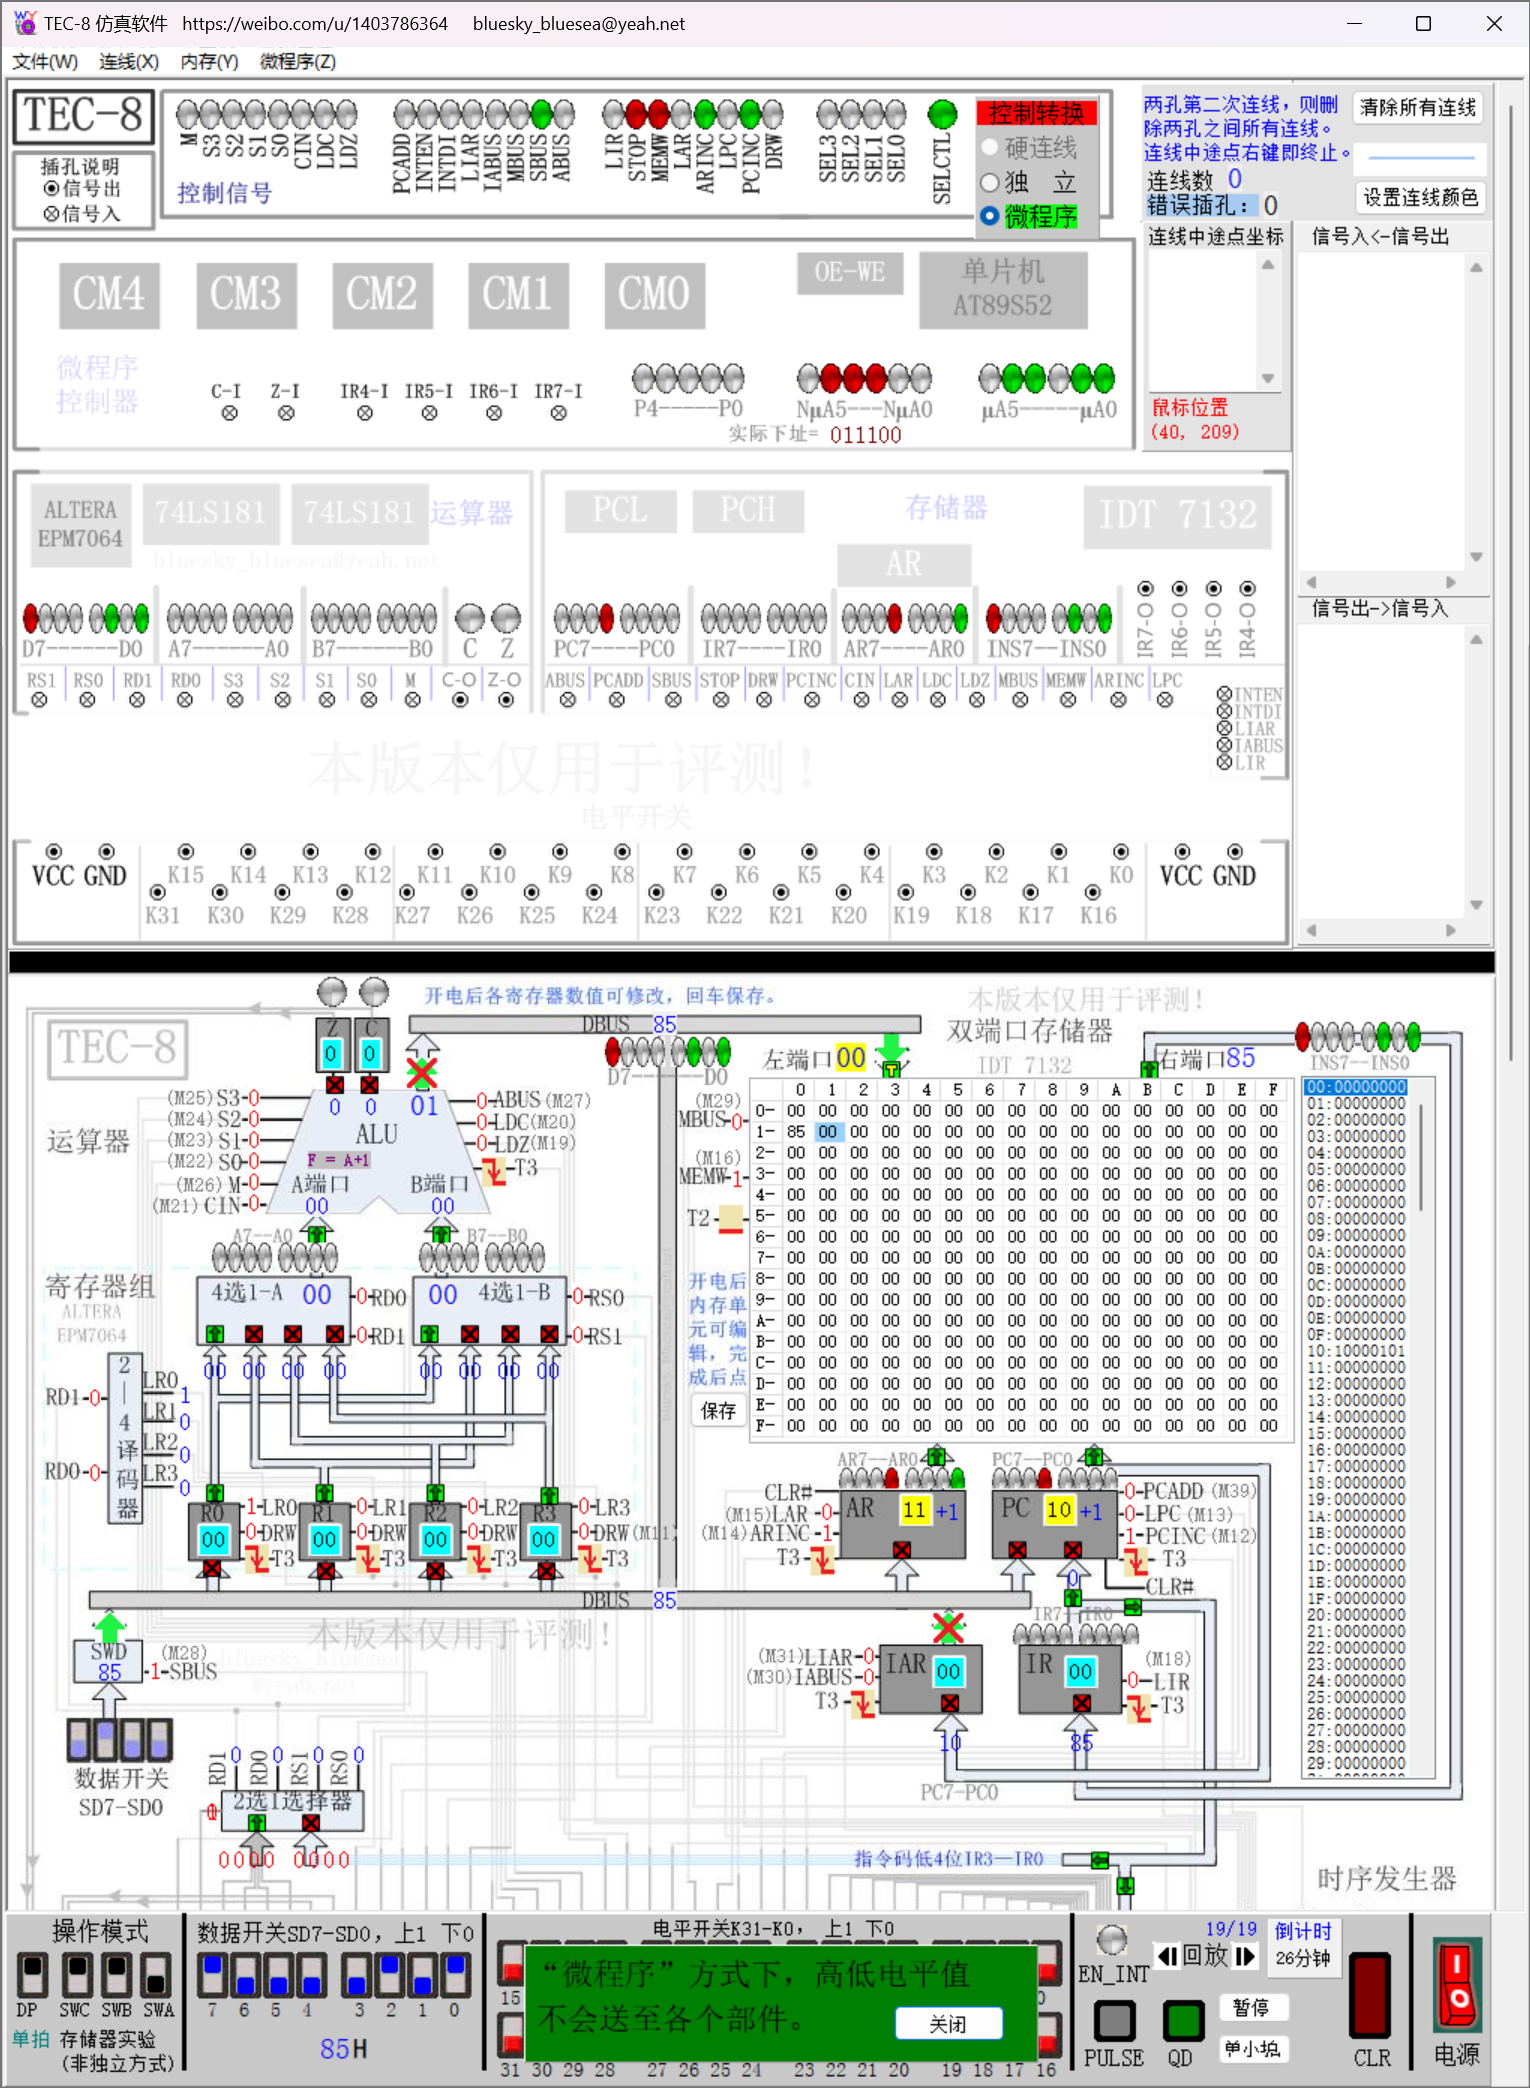
\includegraphics[width=0.3\textwidth]{screenshots/2.1.4.png}
              }
              \subfigure[数据60H]{
                  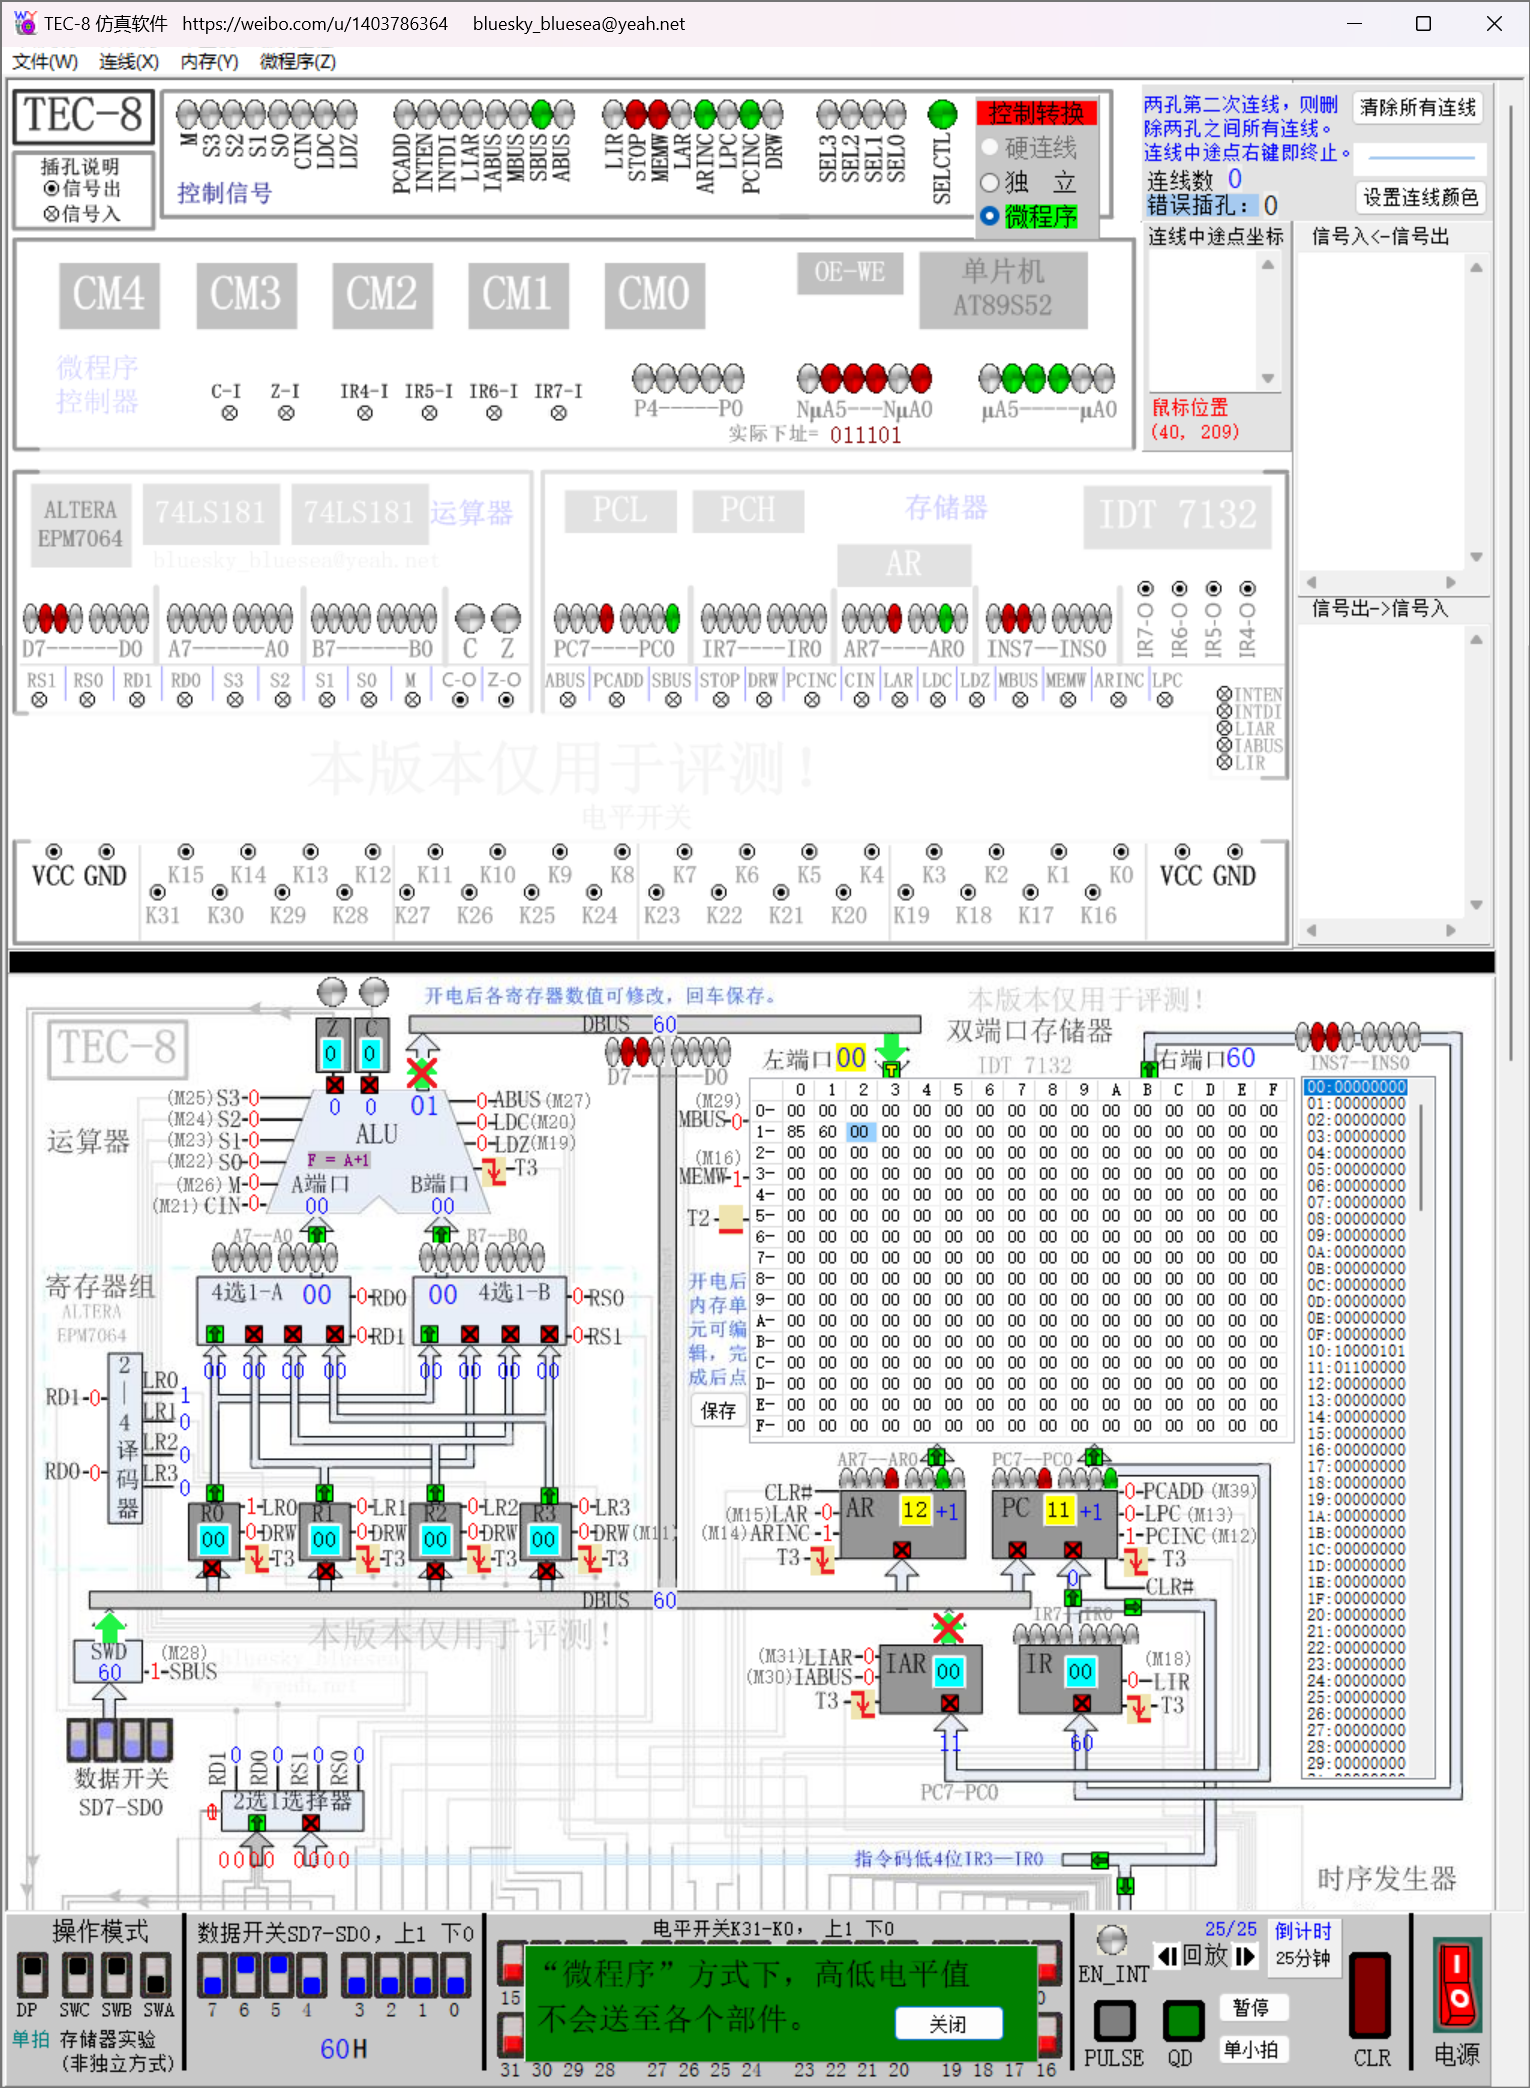
\includegraphics[width=0.3\textwidth]{screenshots/2.1.5.png}
              }
              \subfigure[数据38H]{
                  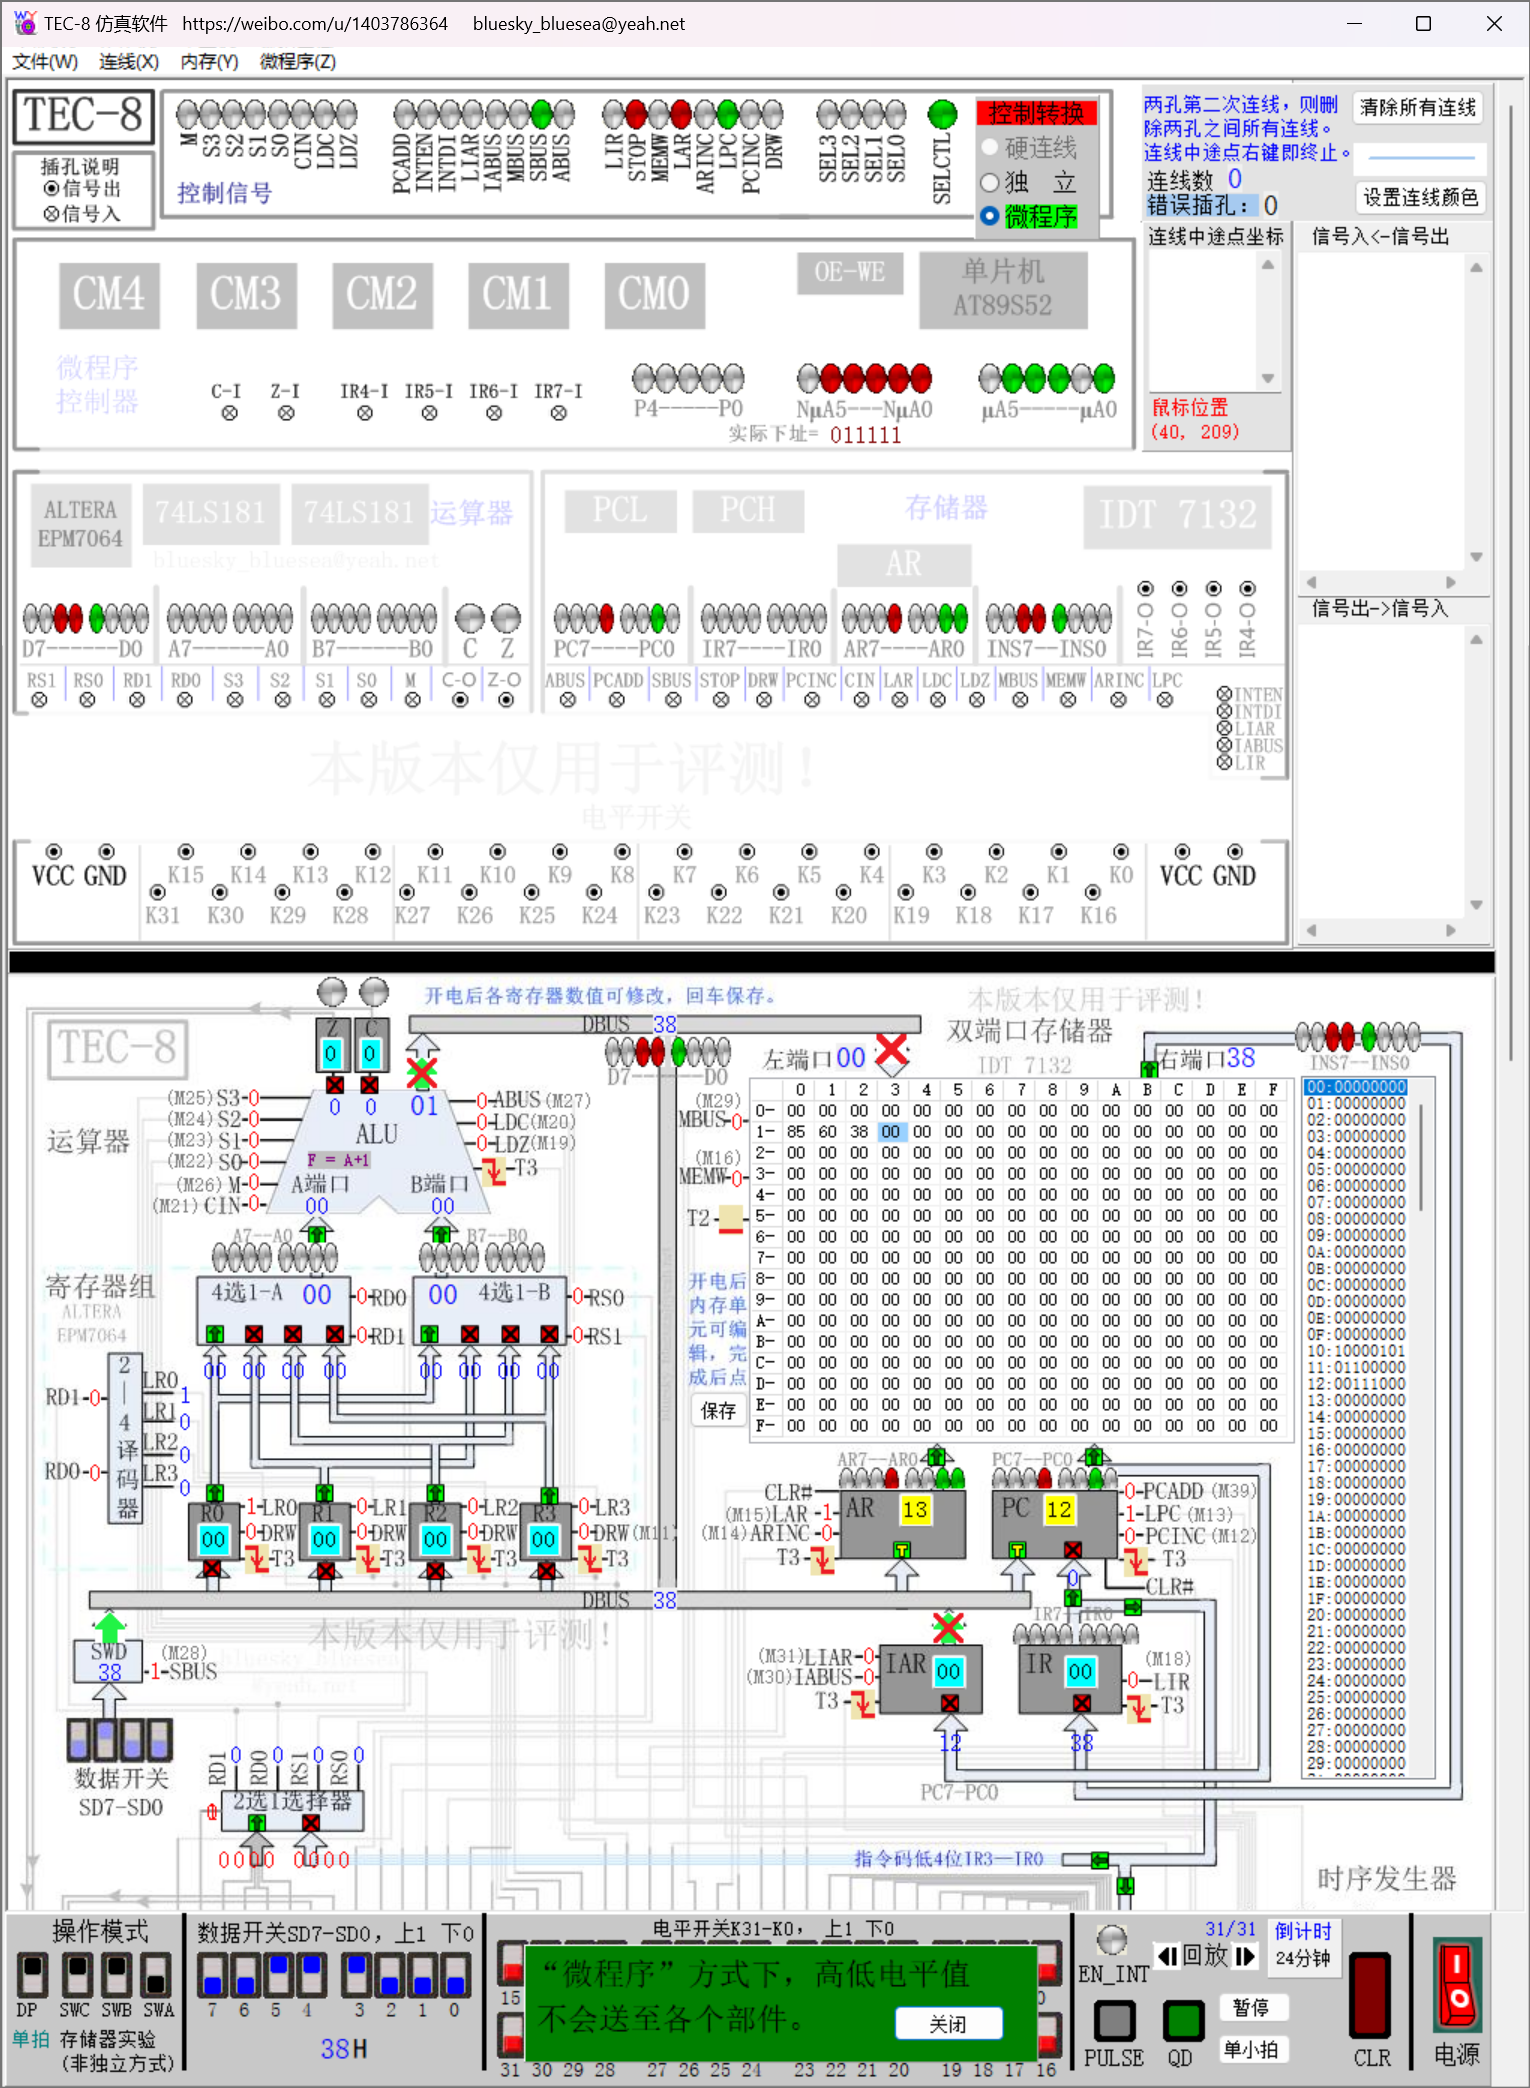
\includegraphics[width=0.3\textwidth]{screenshots/2.1.6.png}
              }
              \caption{数据写入 (微程序)}
              \label{fig:2.1}
          \end{figure}

    \item 重新通过数据开关设置地址为 10H. 按下QD按钮获取存储器中数据. (如图\ref{fig:2.2}所示.)

          \begin{figure}[p]
              \centering
              \subfigure[内存10H]{
                  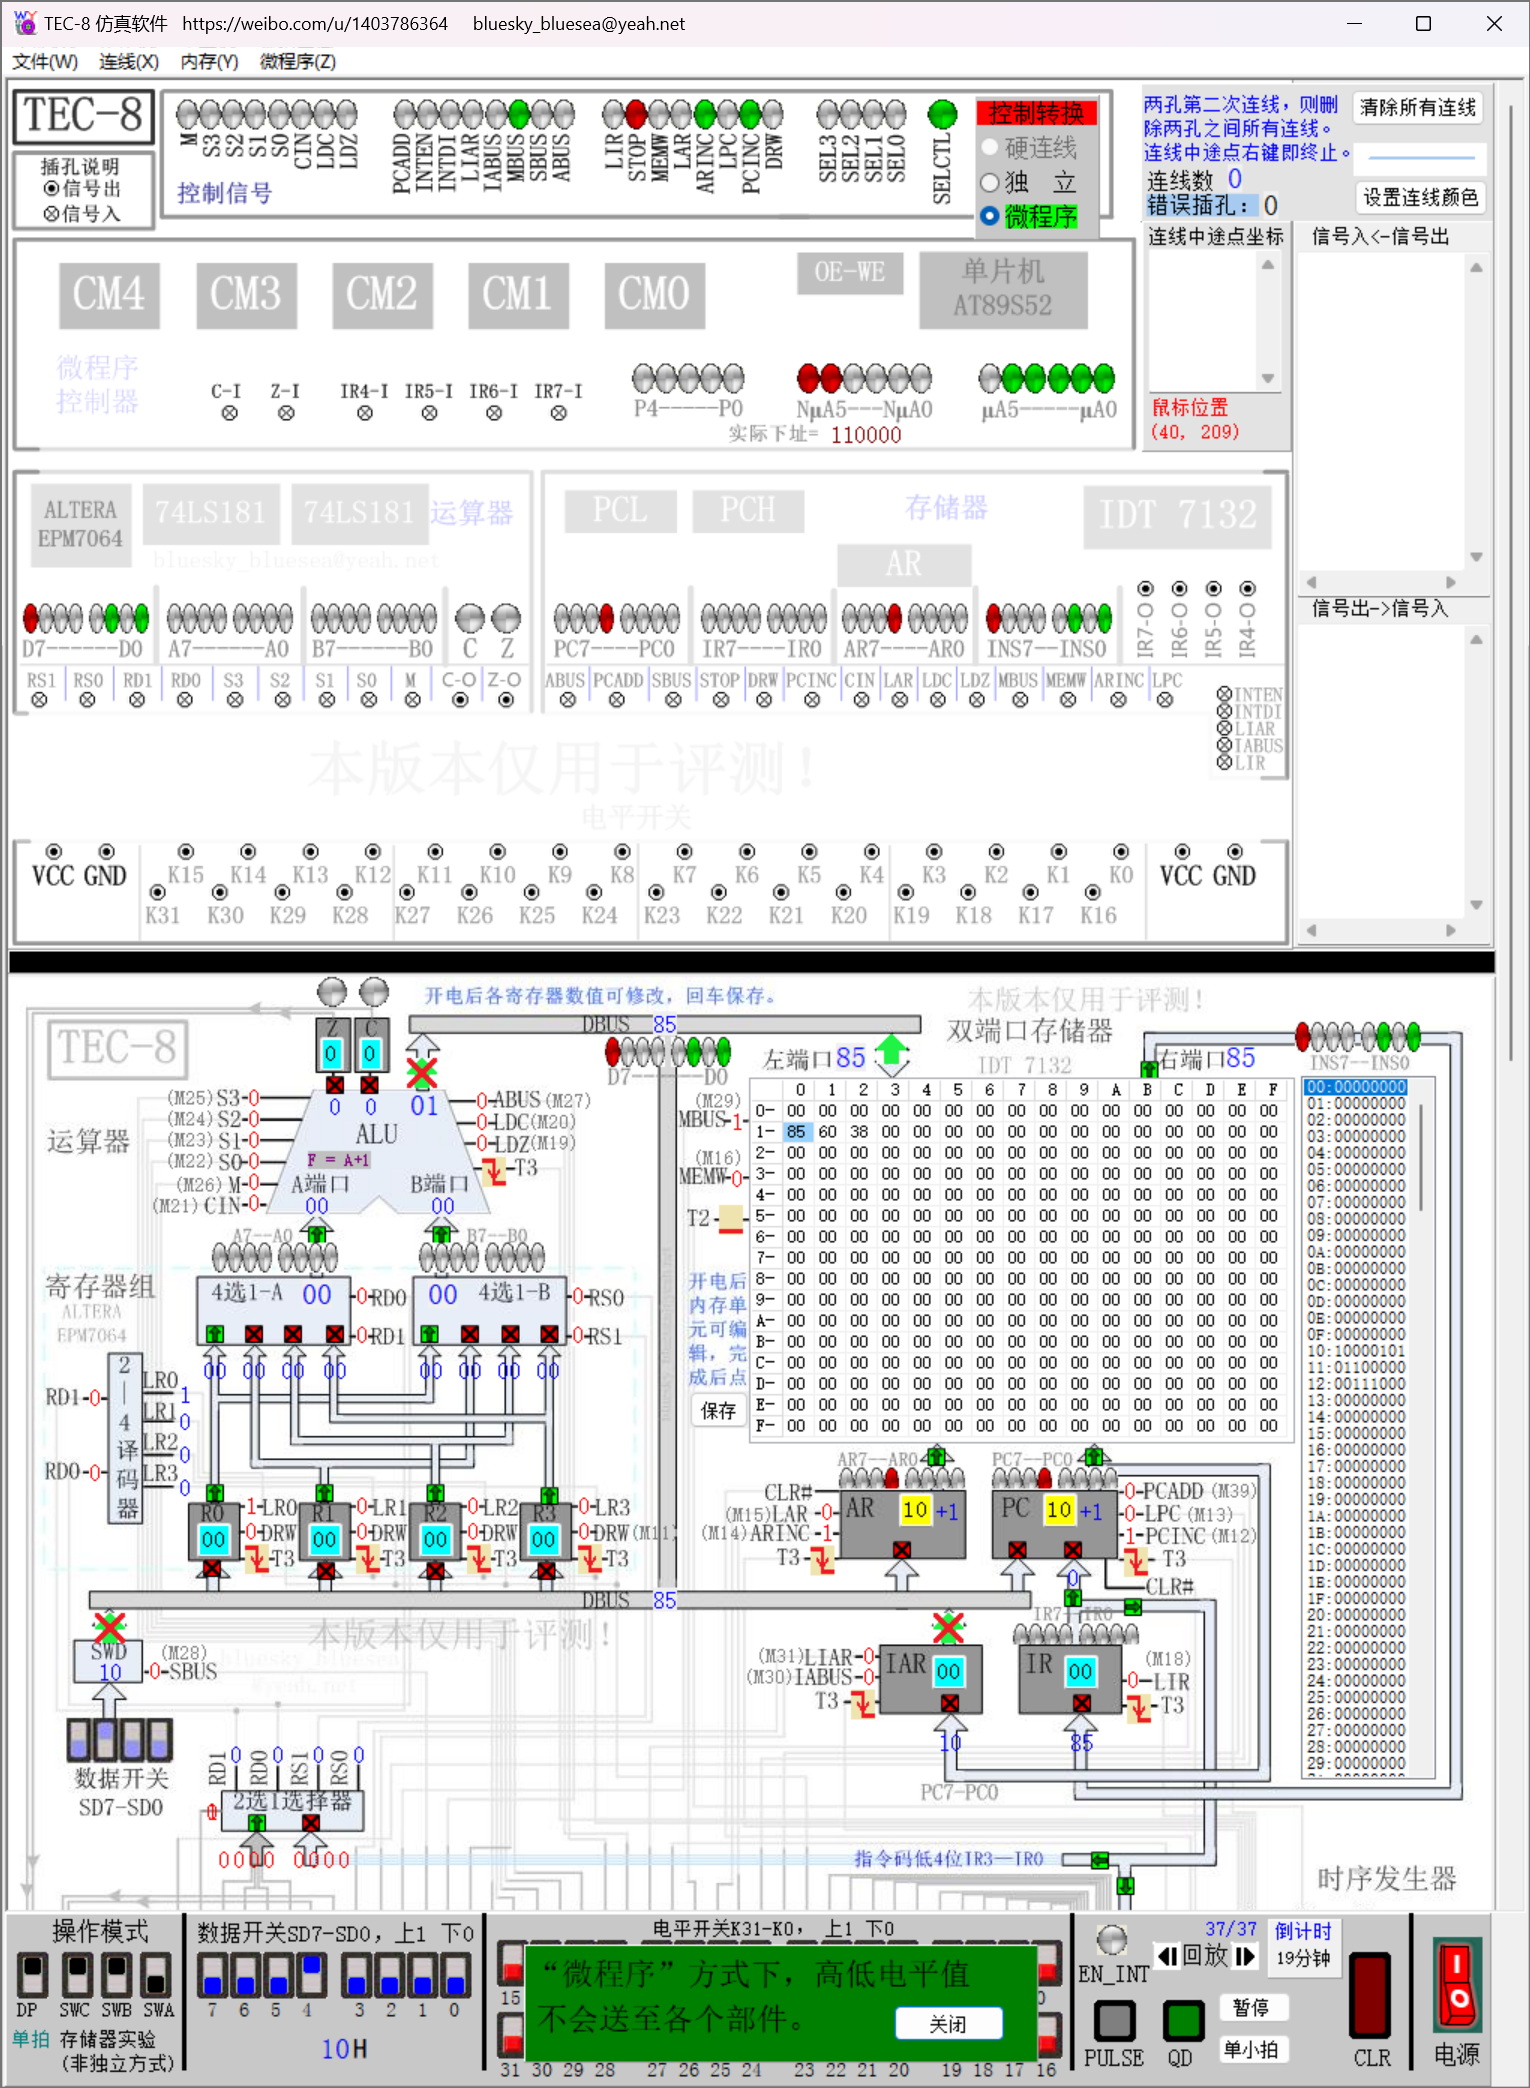
\includegraphics[width=0.3\textwidth]{screenshots/2.1.7.png}
              }
              \subfigure[内存11H]{
                  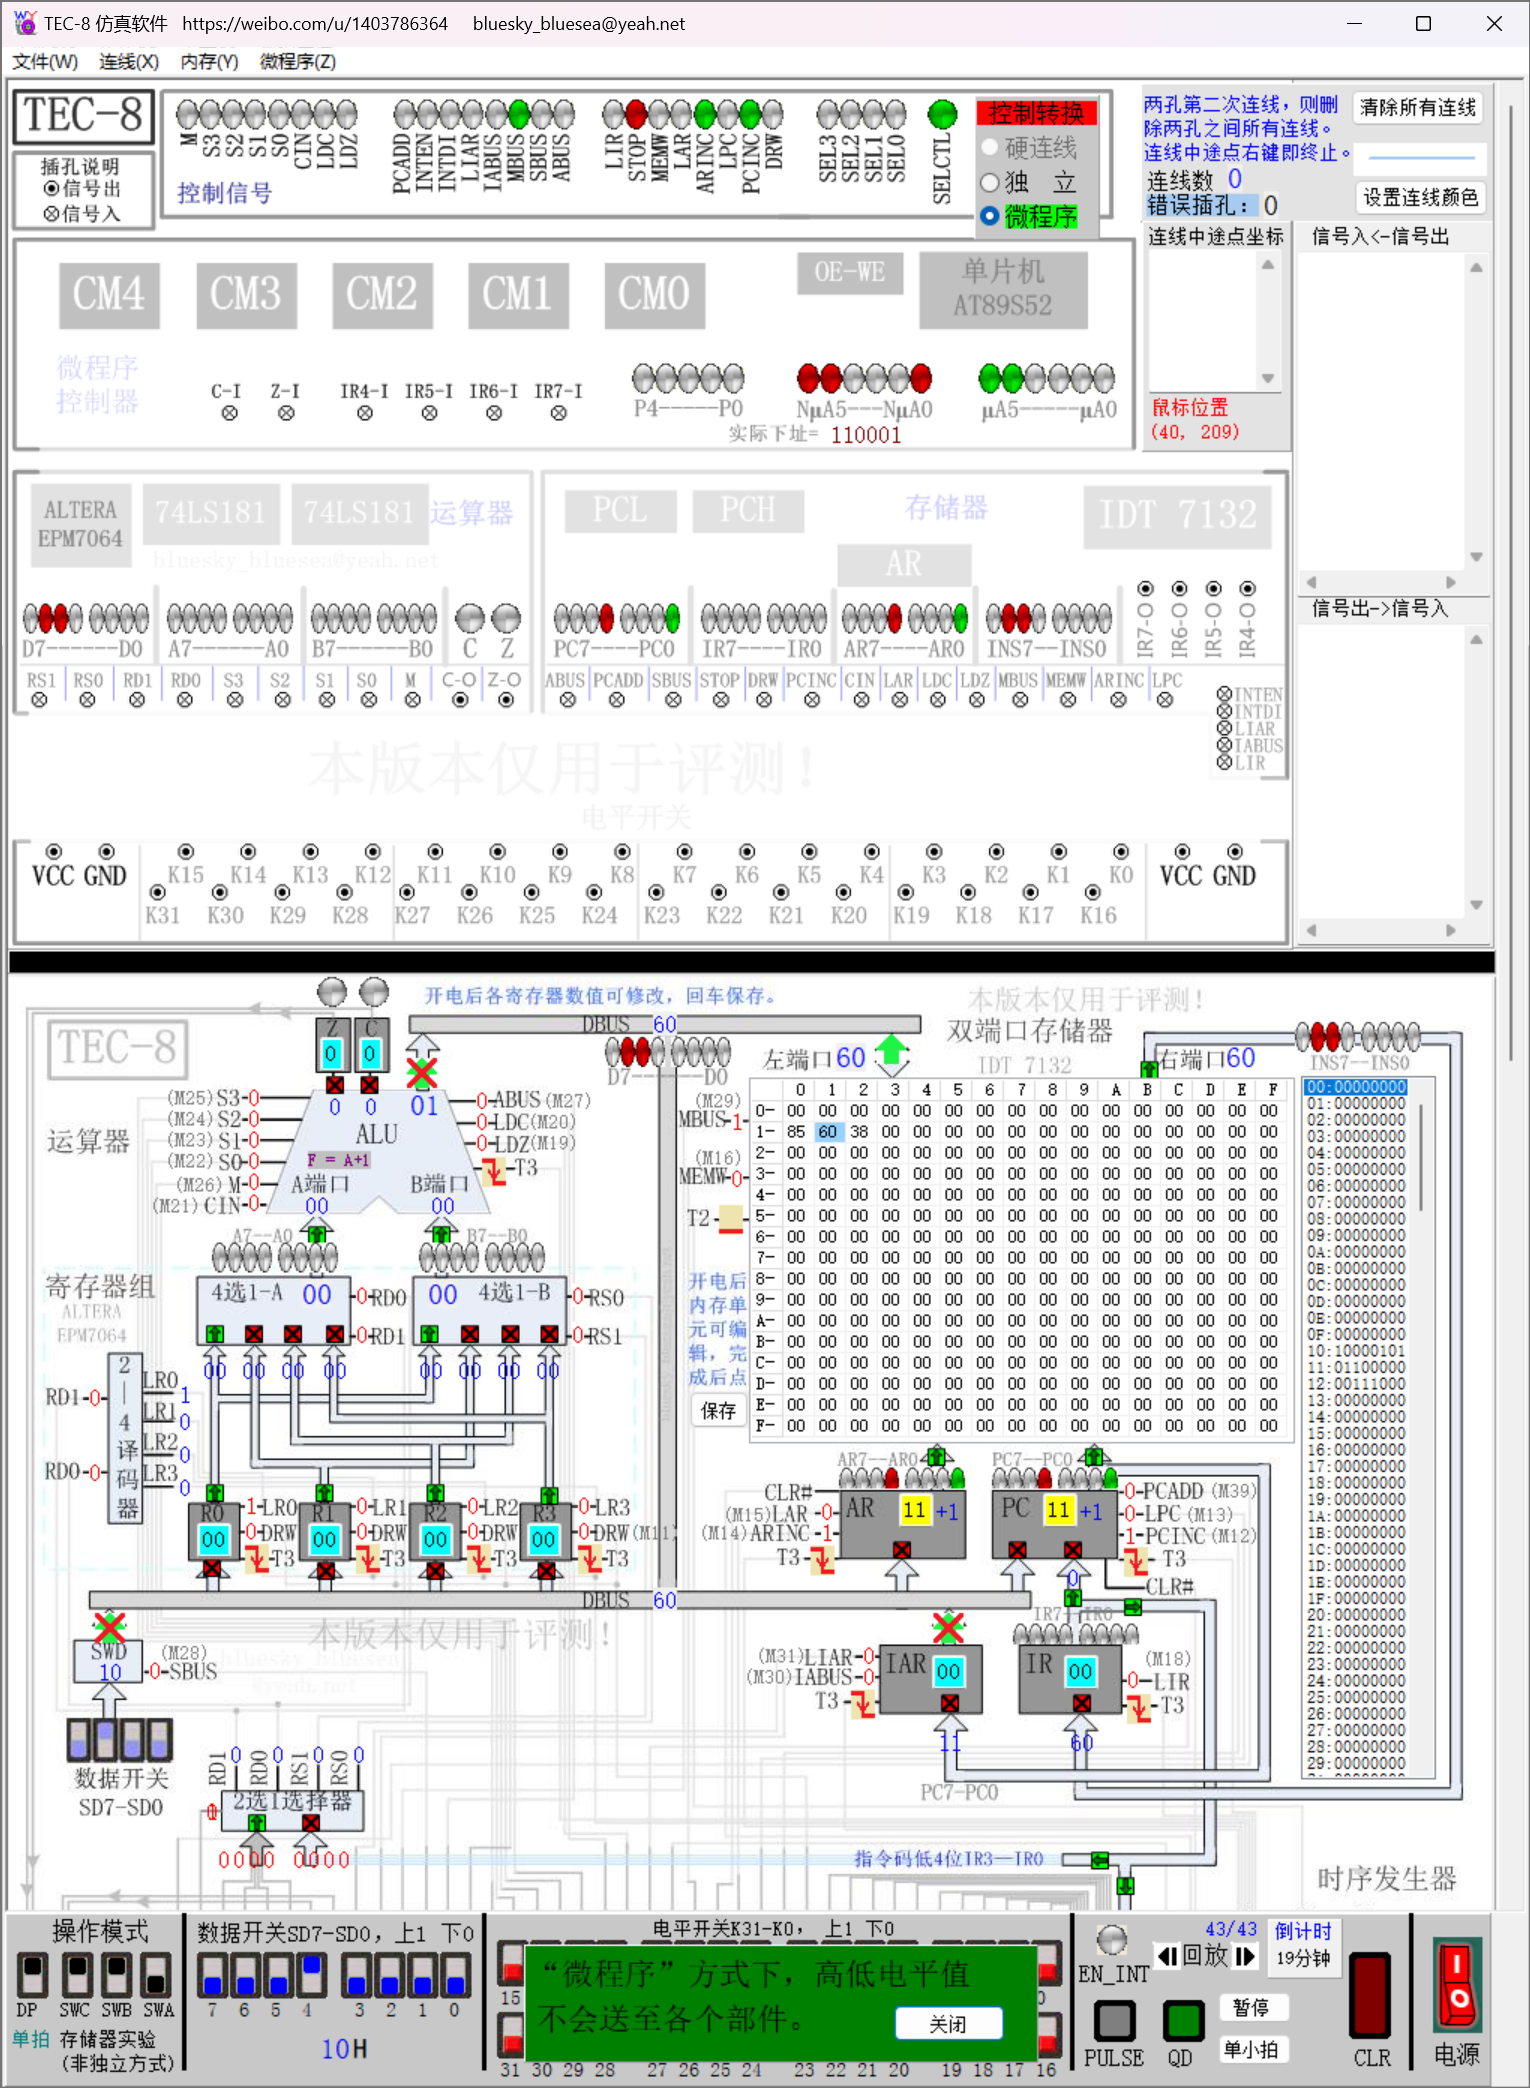
\includegraphics[width=0.3\textwidth]{screenshots/2.1.8.png}
              }
              \subfigure[内存12H]{
                  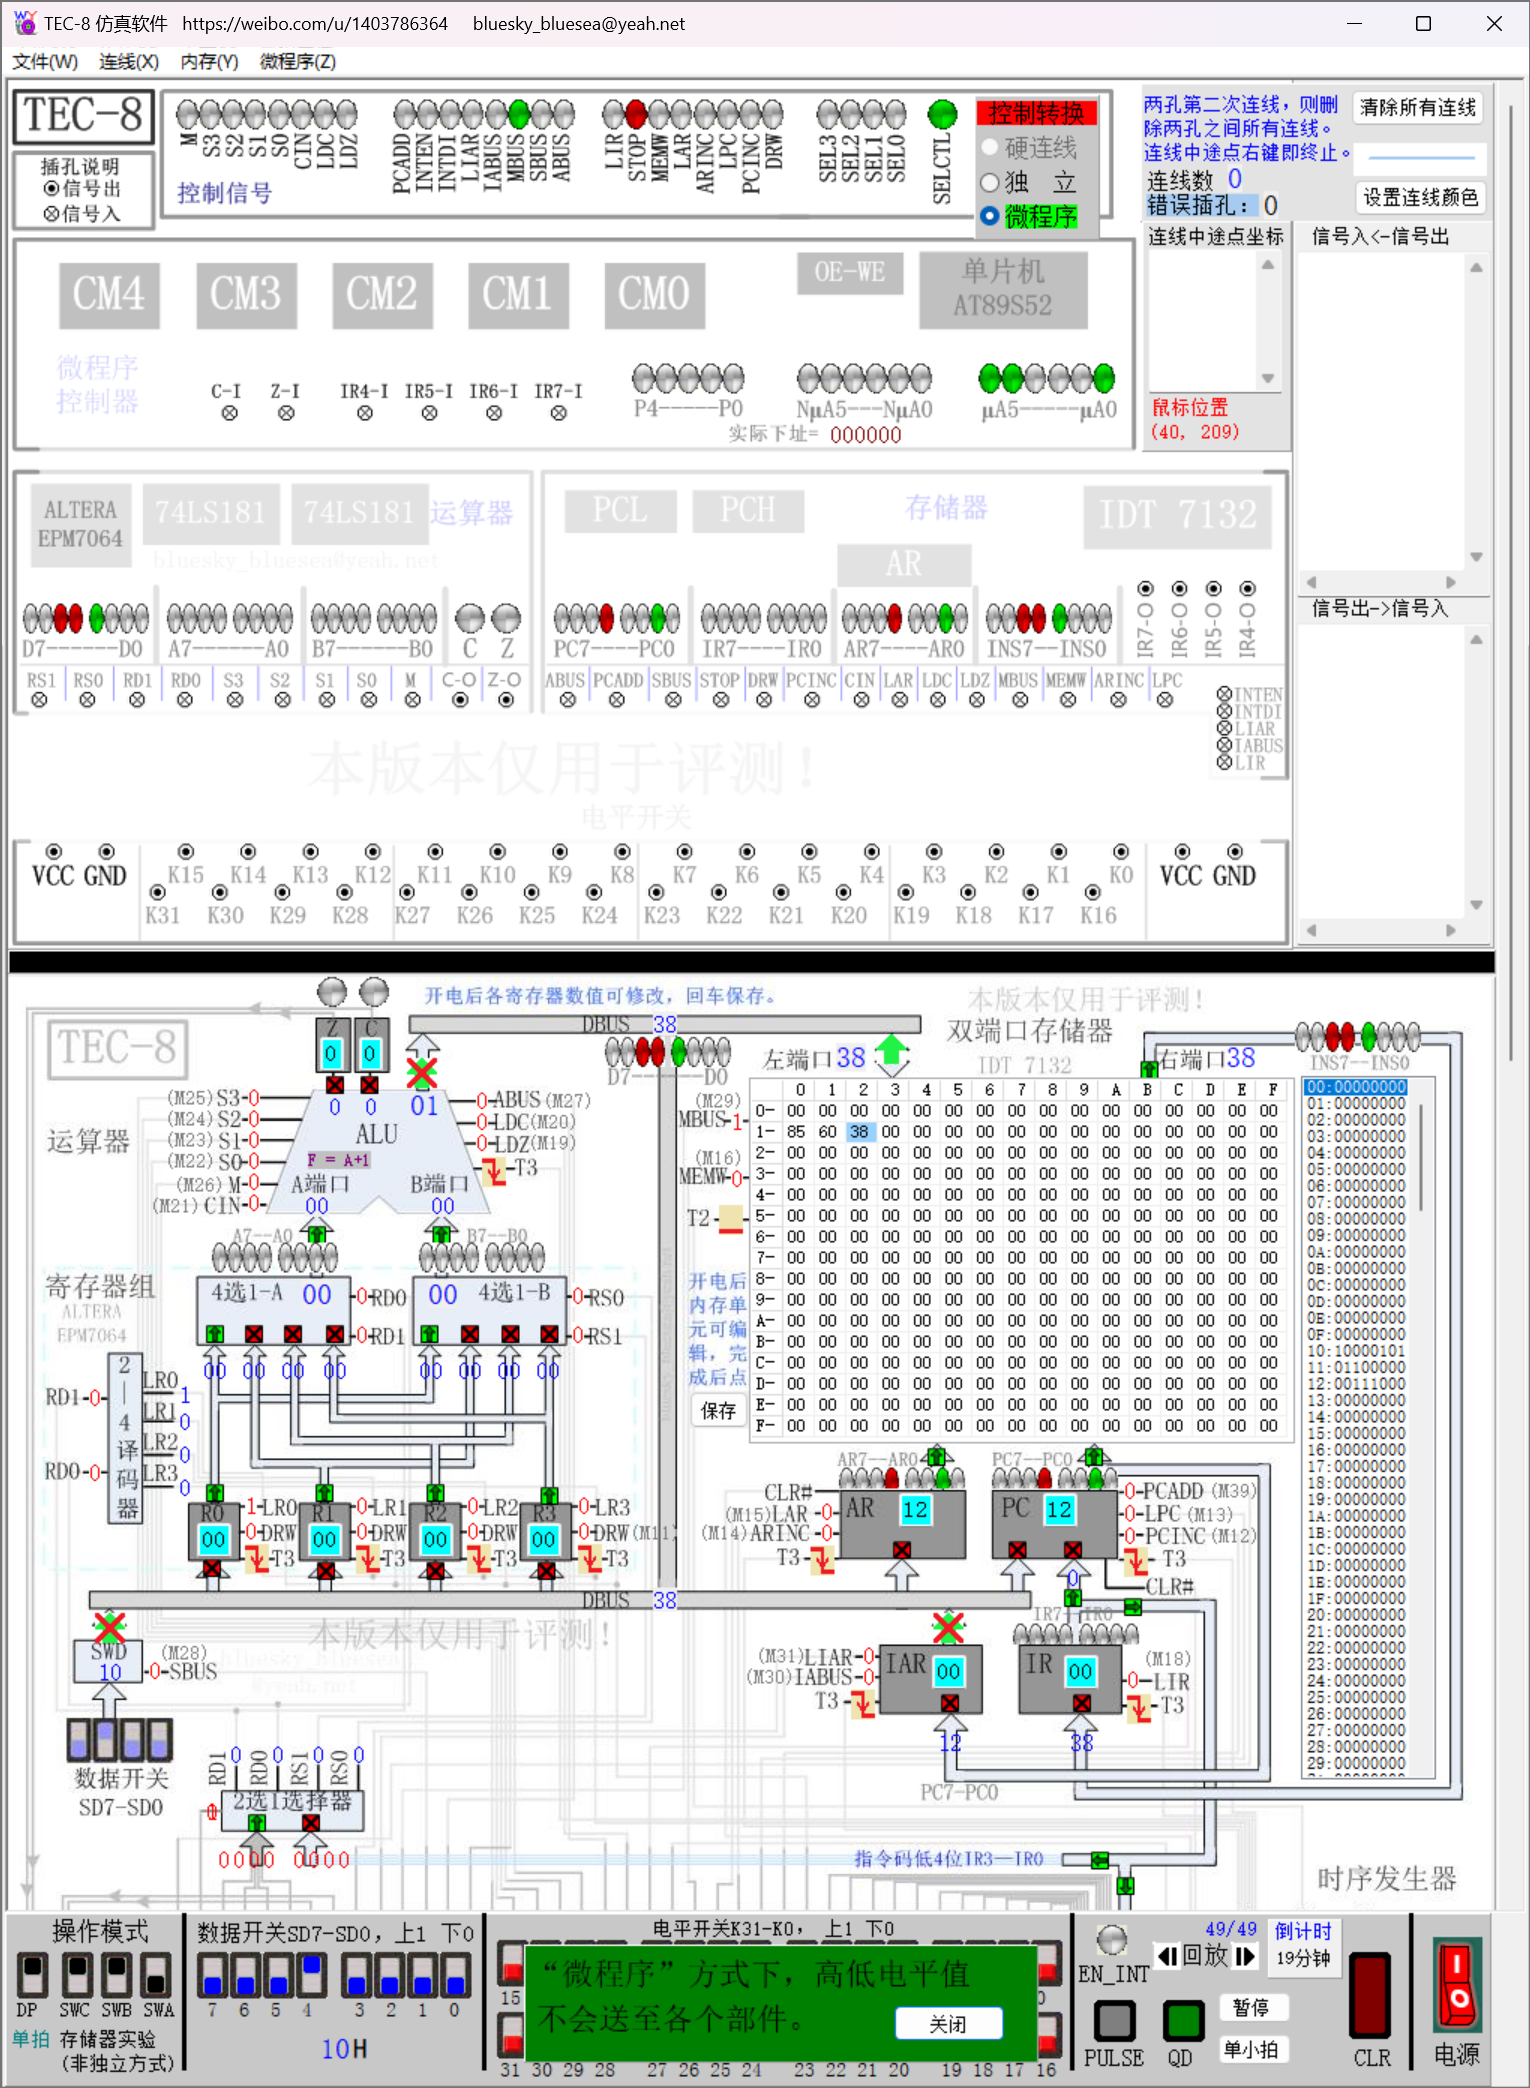
\includegraphics[width=0.3\textwidth]{screenshots/2.1.9.png}
              }
              \caption{数据读取 (微程序)}
              \label{fig:2.2}
          \end{figure}

    \item 实验结果如表\ref{tab:2.1}所示.

          \begin{table}[htb]
              \centering
              \begin{tabular}{cc|cccccc}
                  \Xhline{1pt}
                  \multicolumn{2}{c|}{实验数据} & \multicolumn{6}{c}{实验结果}                                                                                         \\ \hline
                  \multirow{2}{*}{\makecell{左端                                                                                                                 \\口存\\储器\\地址}} & \multirow{2}{*}{\makecell{通过\\左端口\\写入的\\数据}} & \multicolumn{2}{c|}{\makecell{第一次从右\\端口读出的数}} & \multicolumn{4}{c}{同时读出时的读出结果}                                                                                                                                                                                                                                                                                  \\ \cline{3-8}
                                            &                          & \makecell{右端口                                                                         \\存储器\\地址}                      & \multicolumn{1}{c|}{\makecell{读出\\的数}} & \makecell{左端口\\存储器\\地址} & \multicolumn{1}{c|}{\makecell{读出\\的数}} & \makecell{右端口\\存储器\\地址} & \makecell{读出\\的数} \\ \hline
                  10H                       & 85H                      & 10H           & \multicolumn{1}{c|}{00H} & 10H & \multicolumn{1}{c|}{85H} & 10H & 85H \\
                  11H                       & 60H                      & 10H           & \multicolumn{1}{c|}{85H} & 11H & \multicolumn{1}{c|}{60H} & 11H & 60H \\
                  12H                       & 38H                      & 11H           & \multicolumn{1}{c|}{60H} & 12H & \multicolumn{1}{c|}{38H} & 12H & 38H \\ \Xhline{1pt}
              \end{tabular}
              \caption{实验结果}
              \label{tab:2.1}
          \end{table}

\end{enumerate}

\subsection{独立模式}

\begin{enumerate}

    \item 完成实验相关连线.

    \item 控制相应开关, 先后完成相关数据的写入和读取操作. (如图\ref{fig:2.3}所示.)

          \begin{figure}[hp]
              \centering
              \subfigure[写入数据85H]{
                  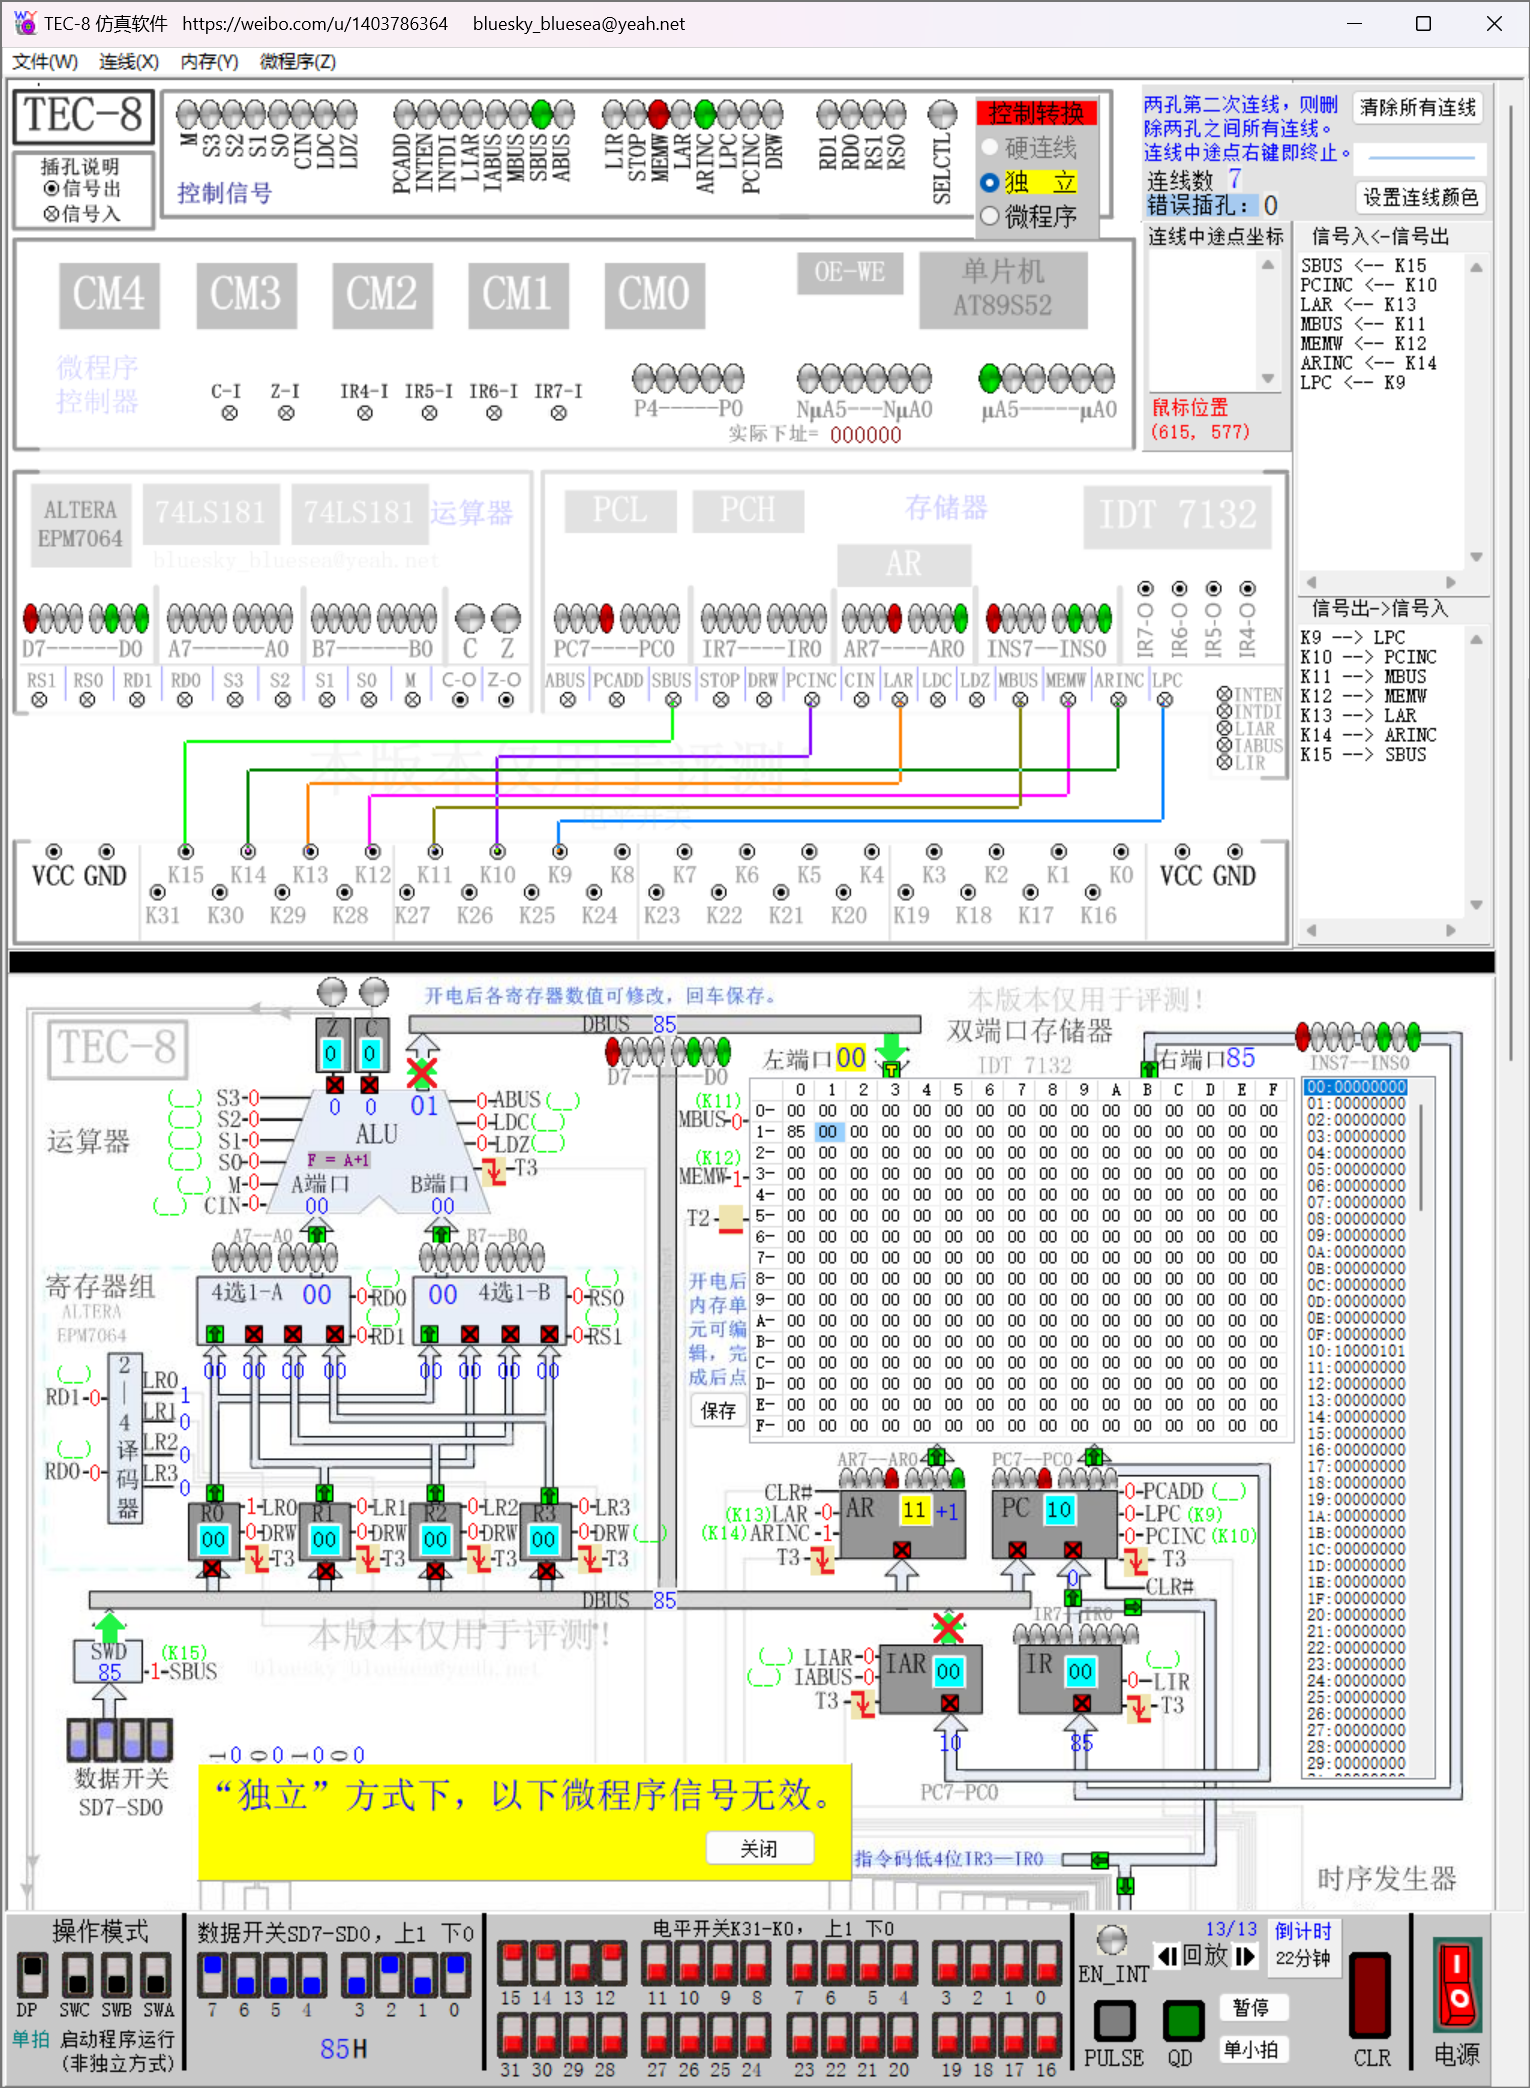
\includegraphics[width=0.3\textwidth]{screenshots/2.2.3.png}
              }
              \subfigure[写入数据60H]{
                  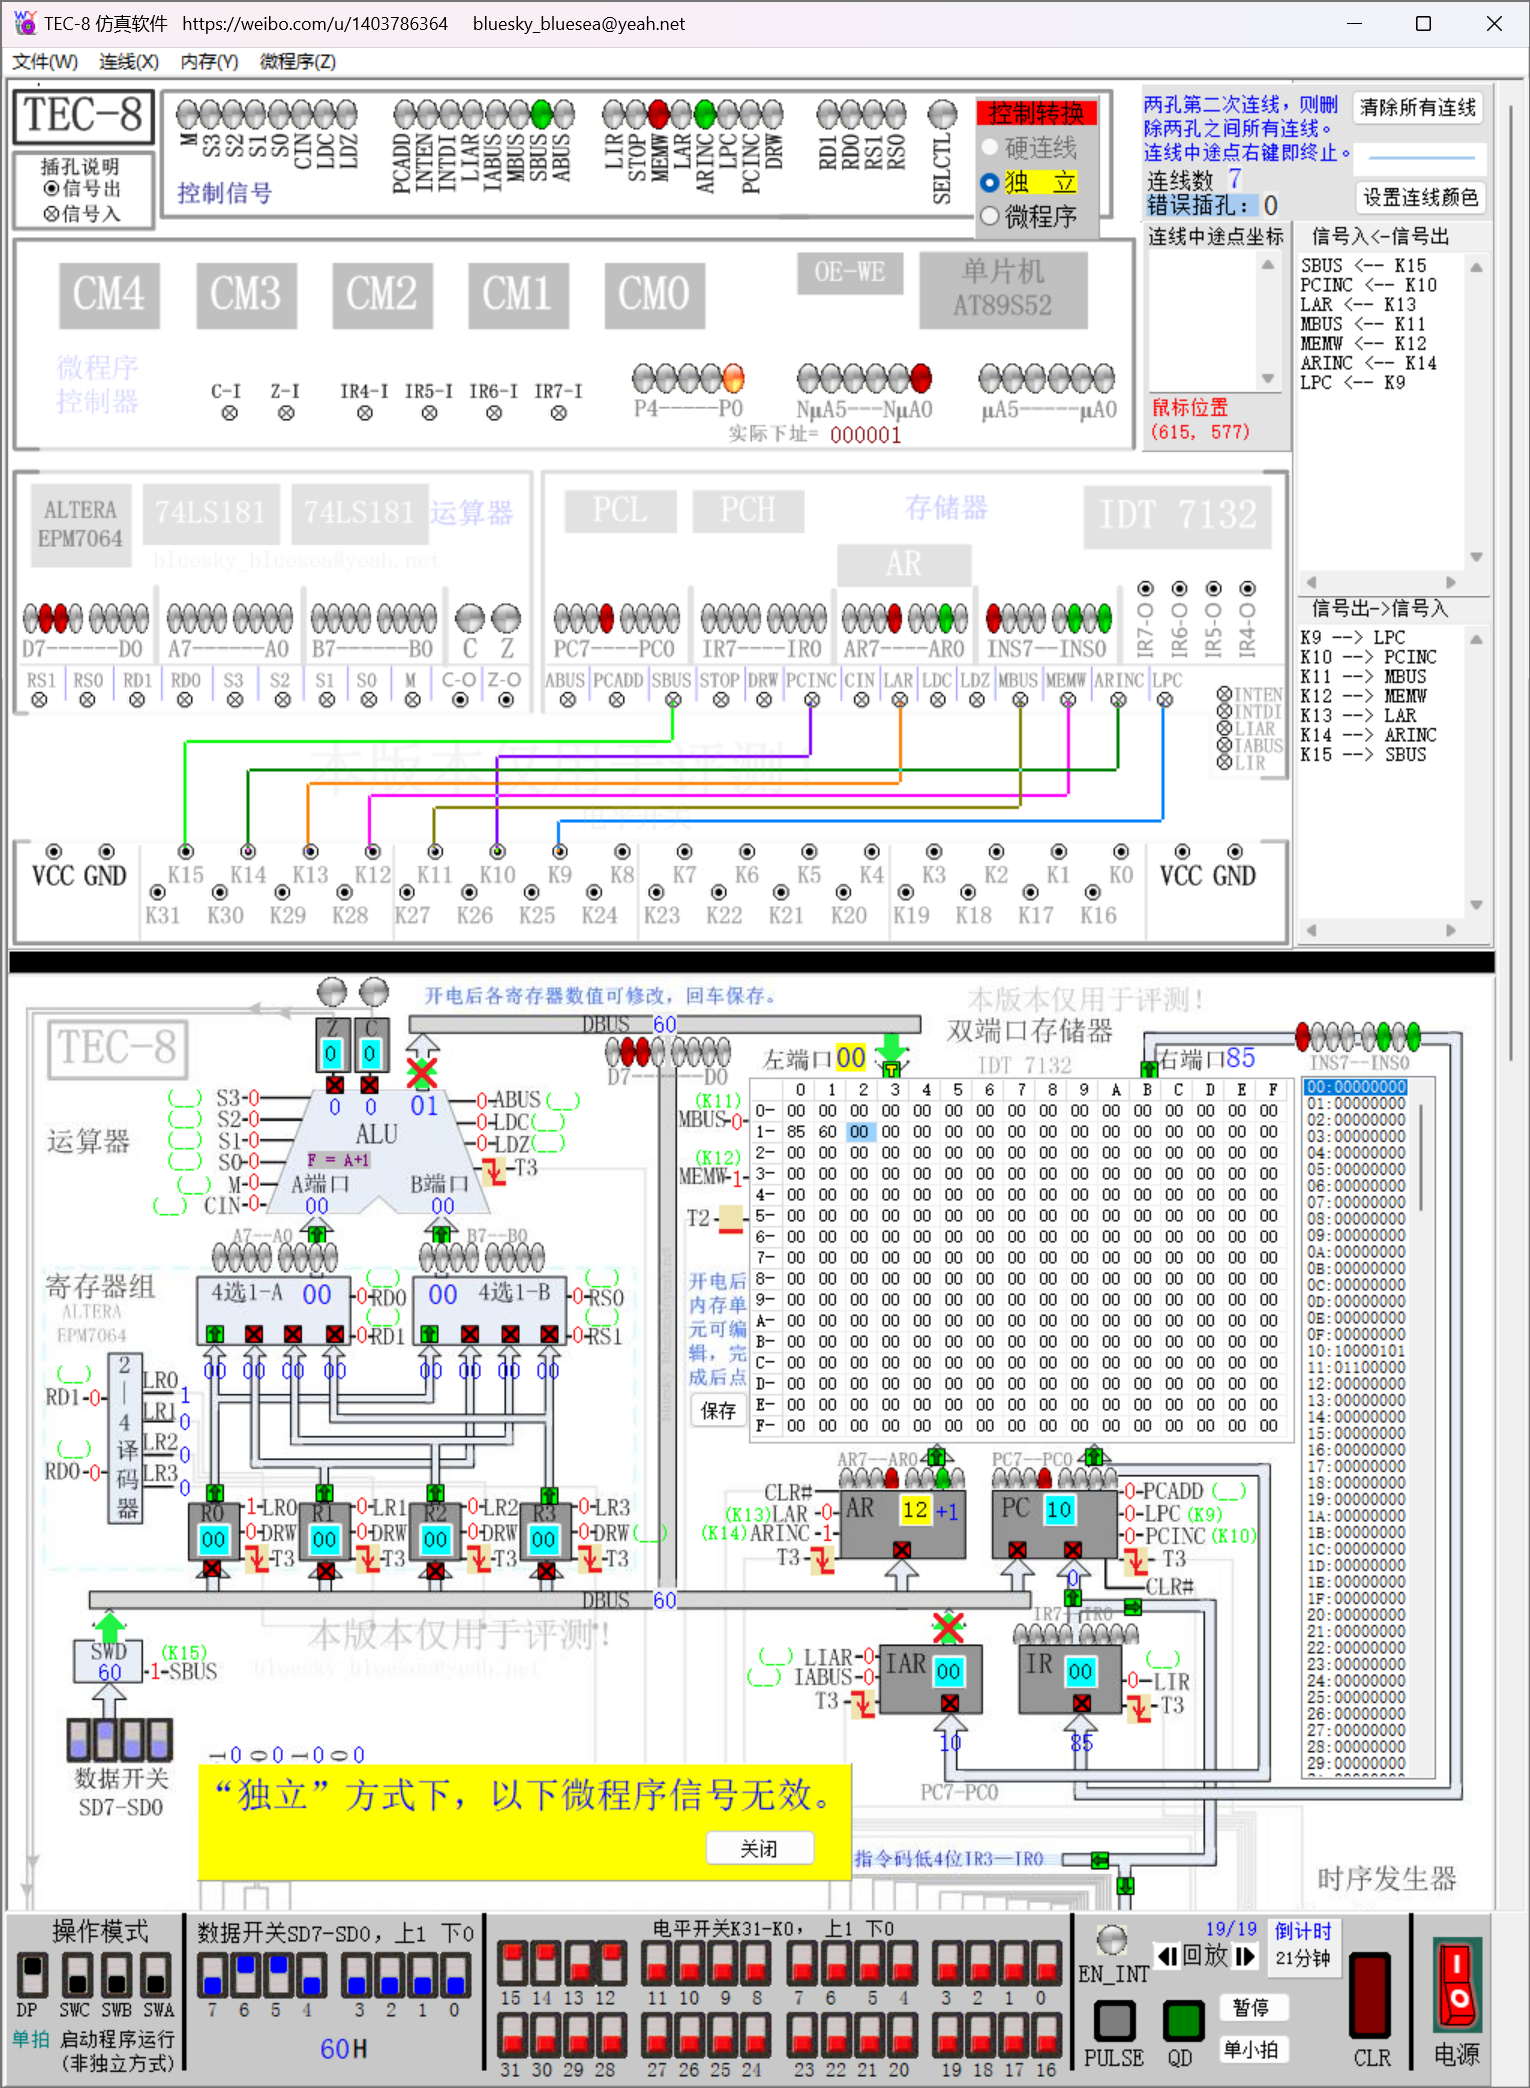
\includegraphics[width=0.3\textwidth]{screenshots/2.2.4.png}
              }
              \subfigure[写入数据38H]{
                  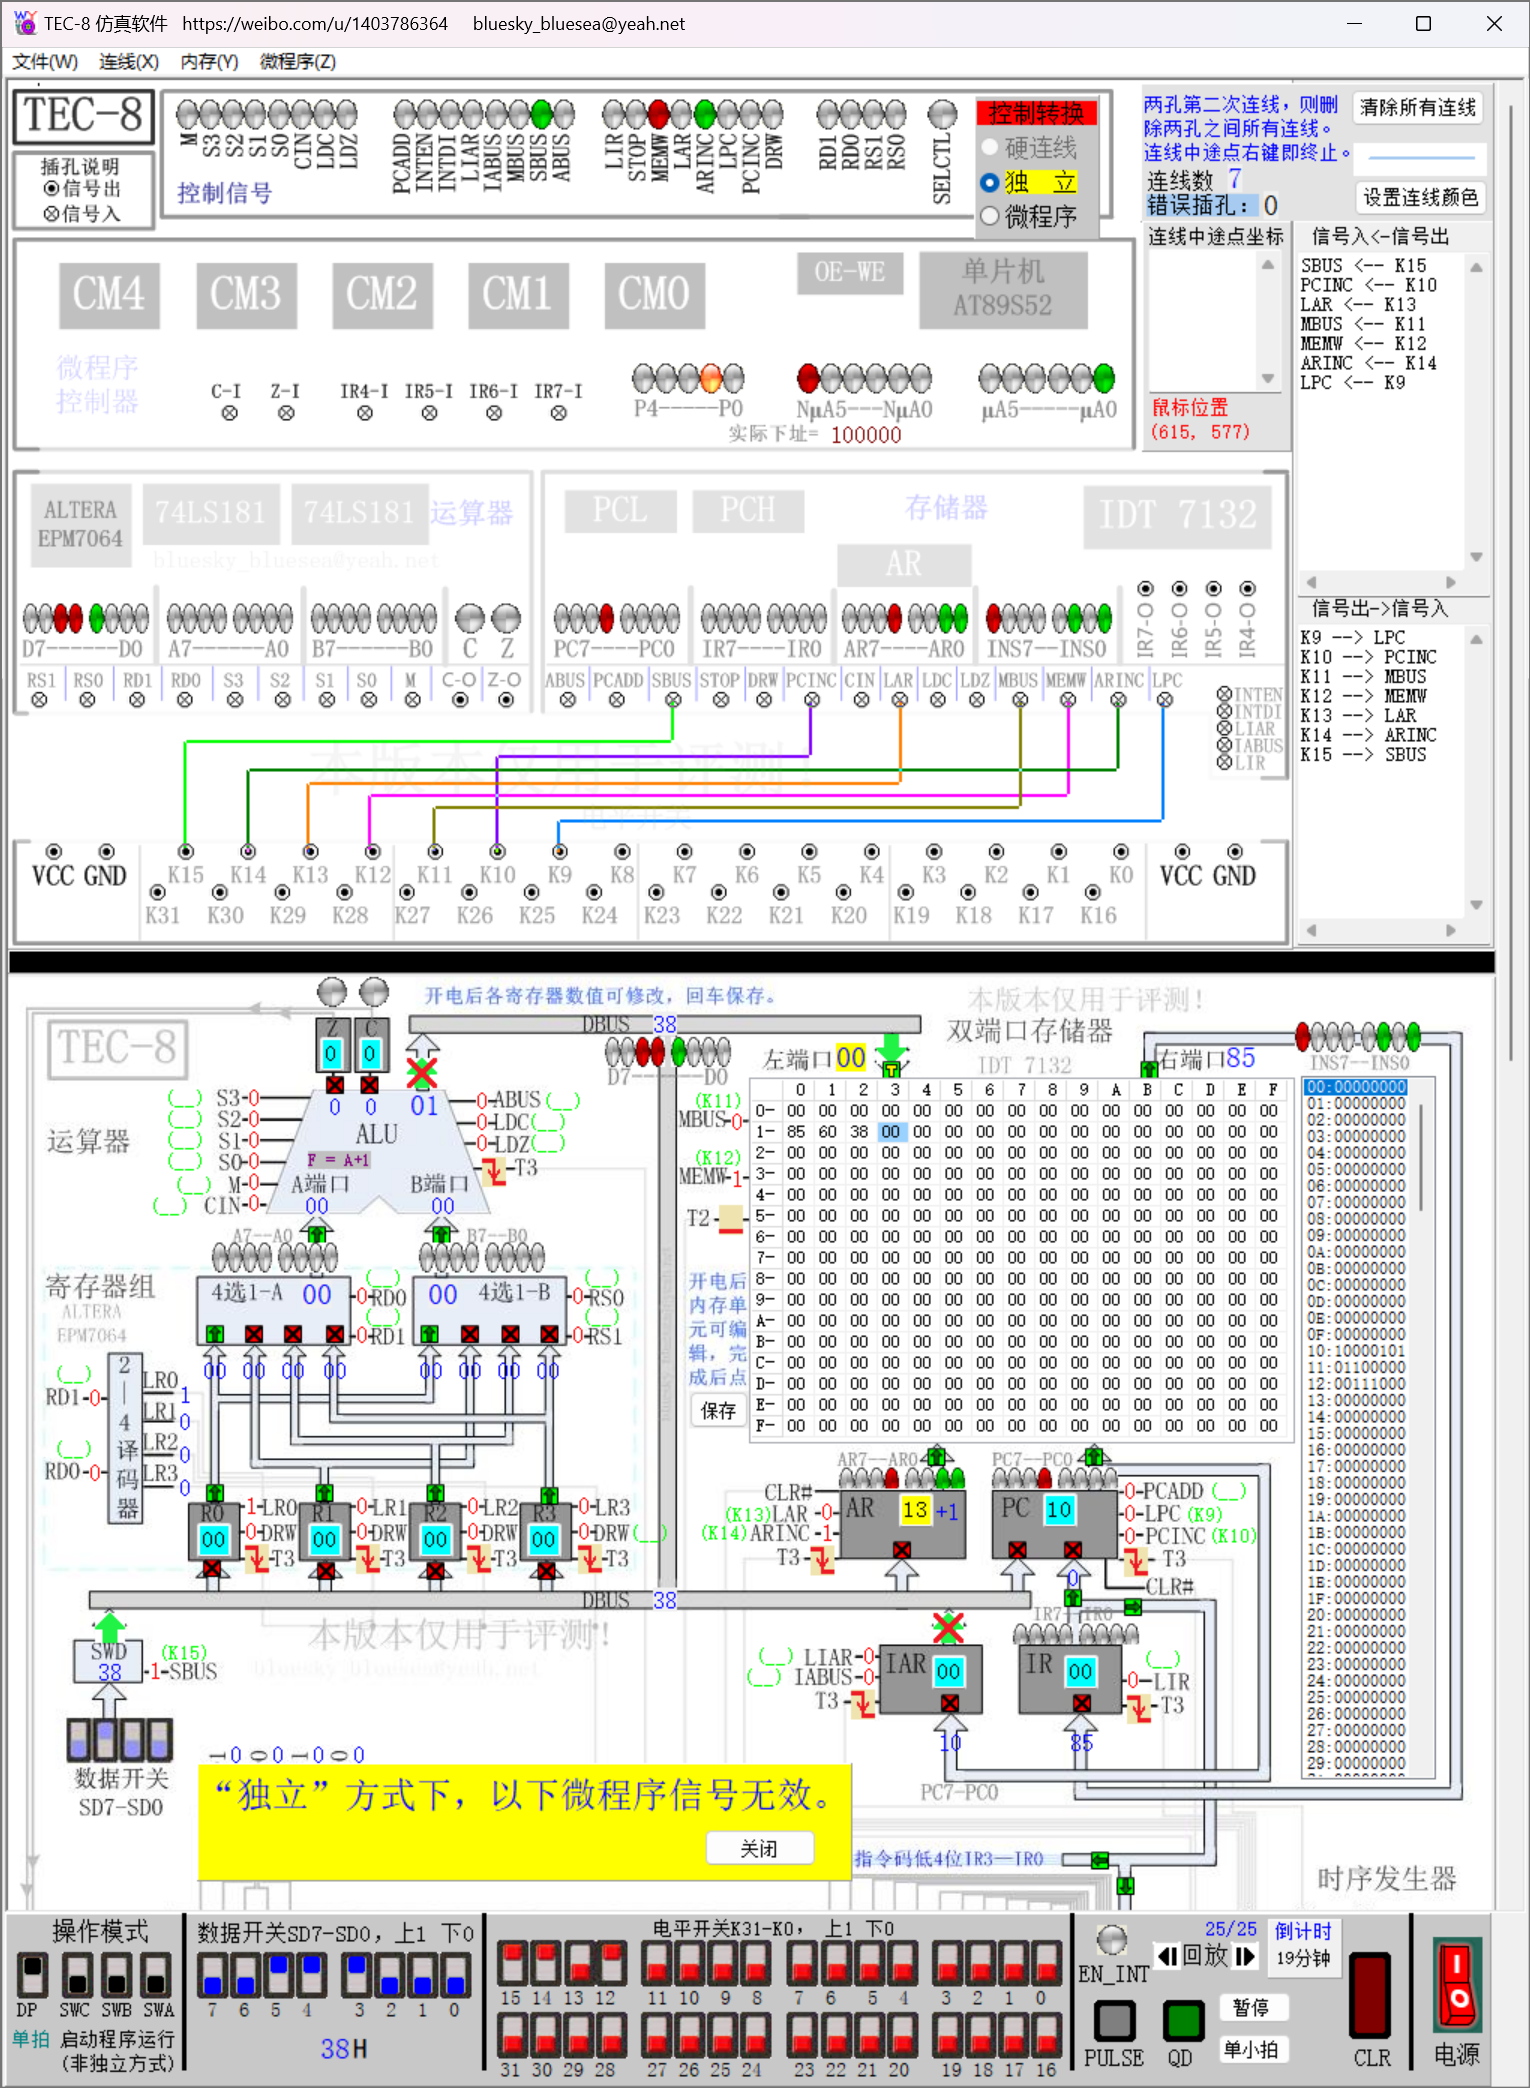
\includegraphics[width=0.3\textwidth]{screenshots/2.2.5.png}
              }
              \\
              \subfigure[读取内存10H]{
                  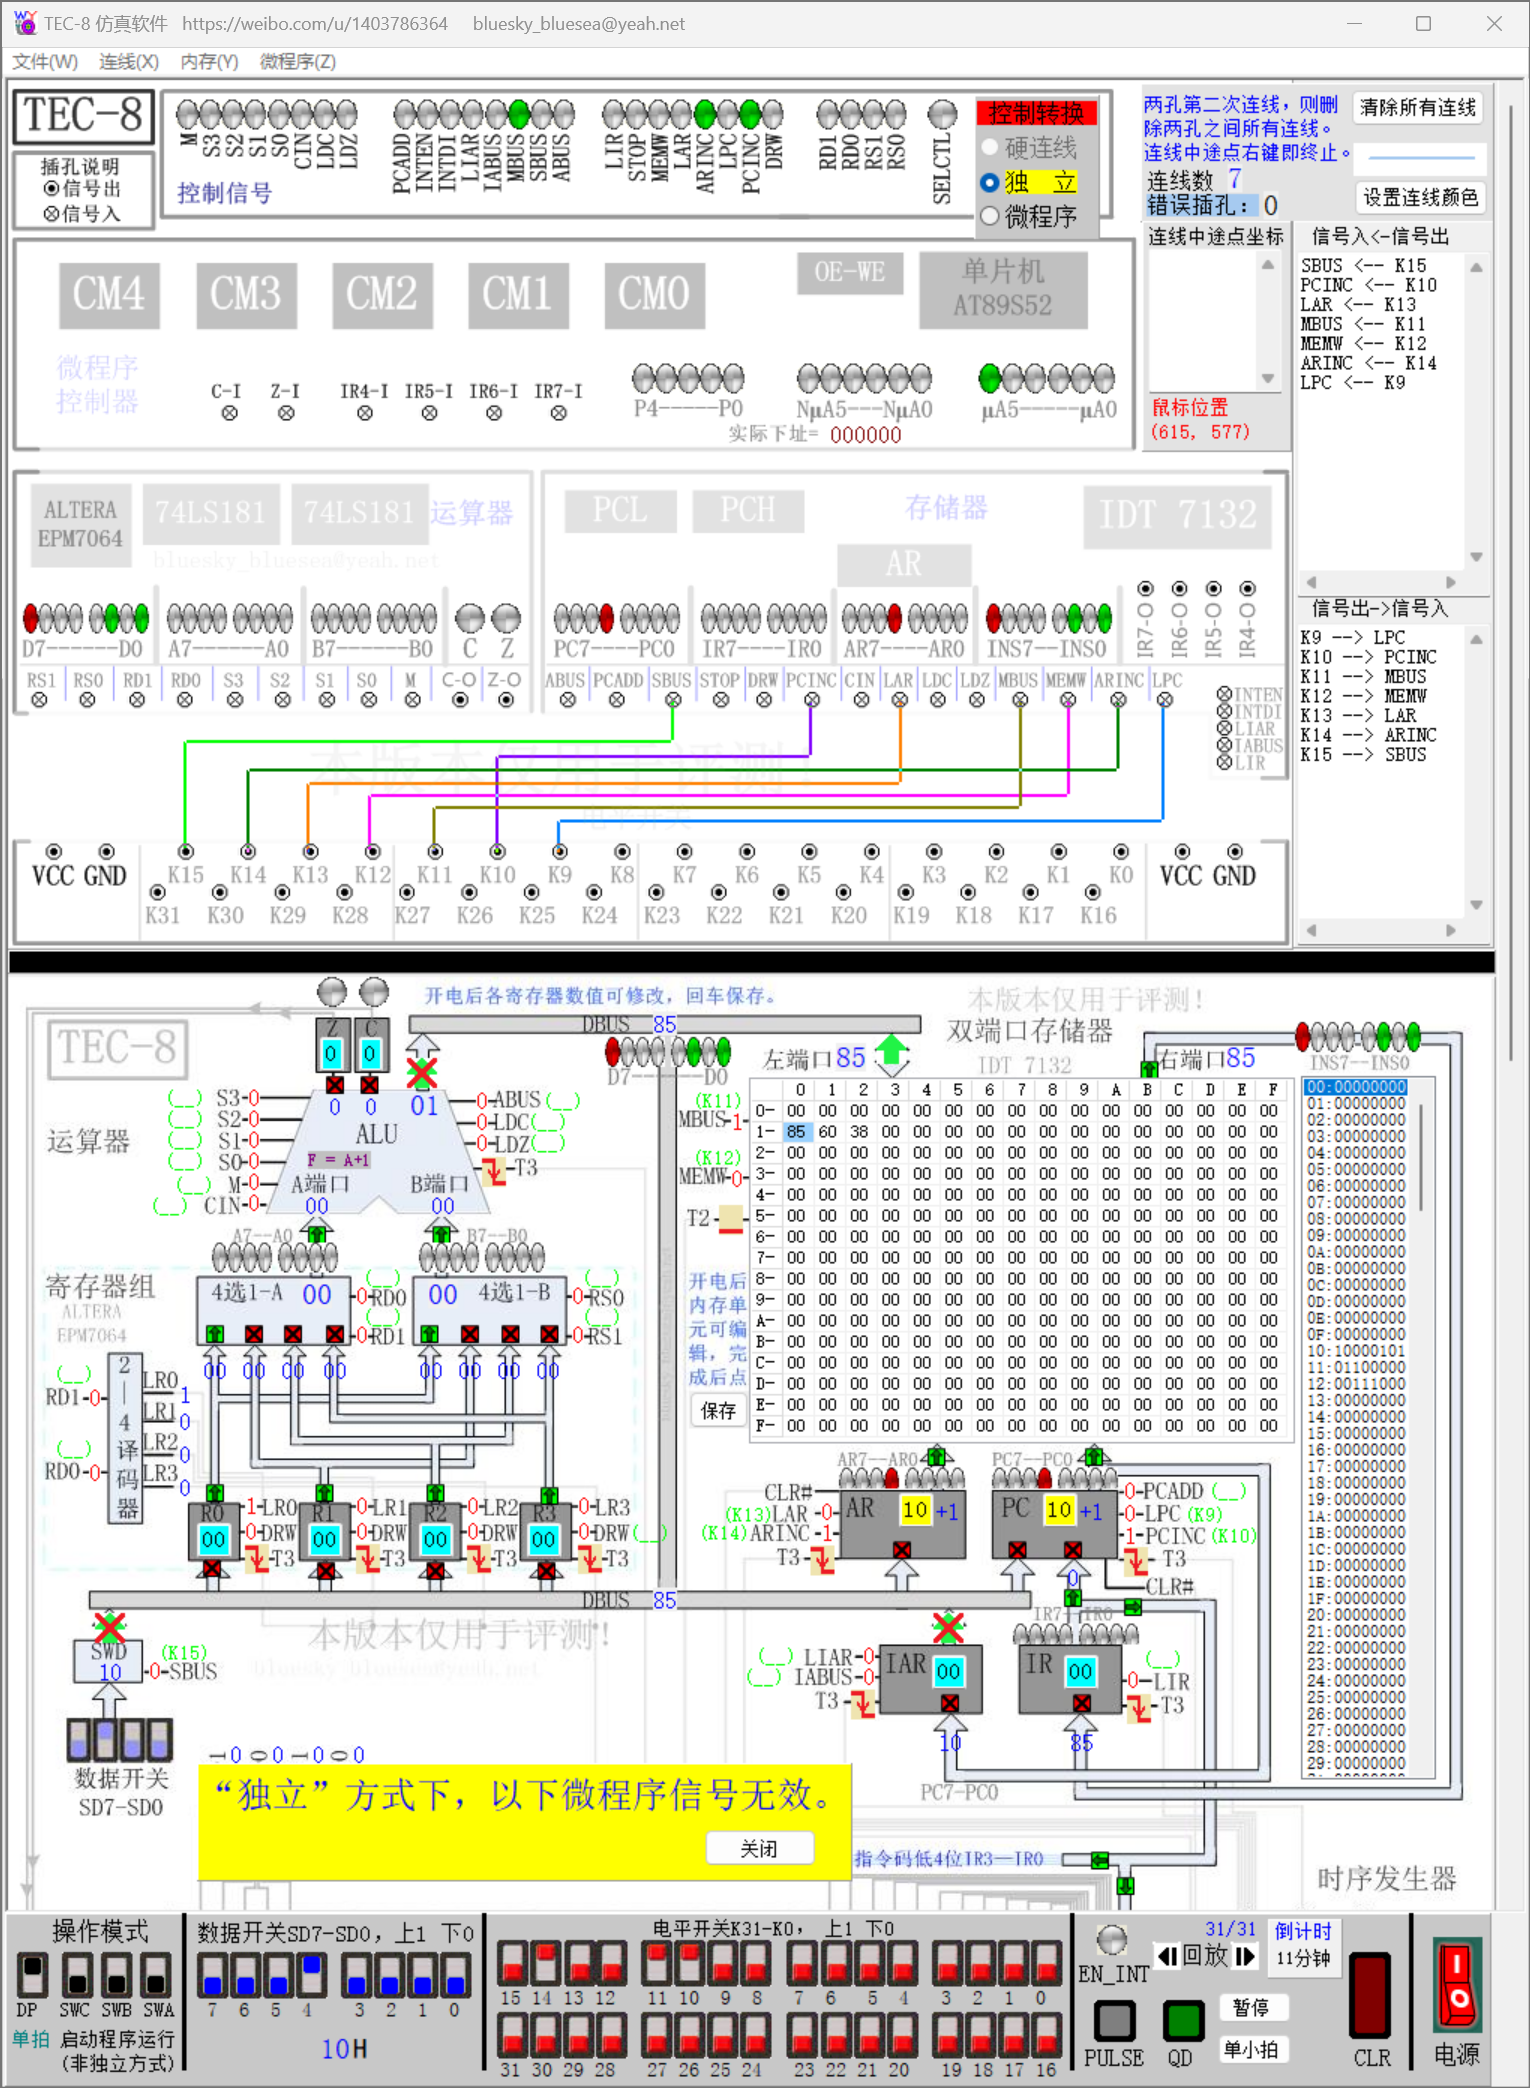
\includegraphics[width=0.3\textwidth]{screenshots/2.2.7.png}
              }
              \subfigure[读取内存11H]{
                  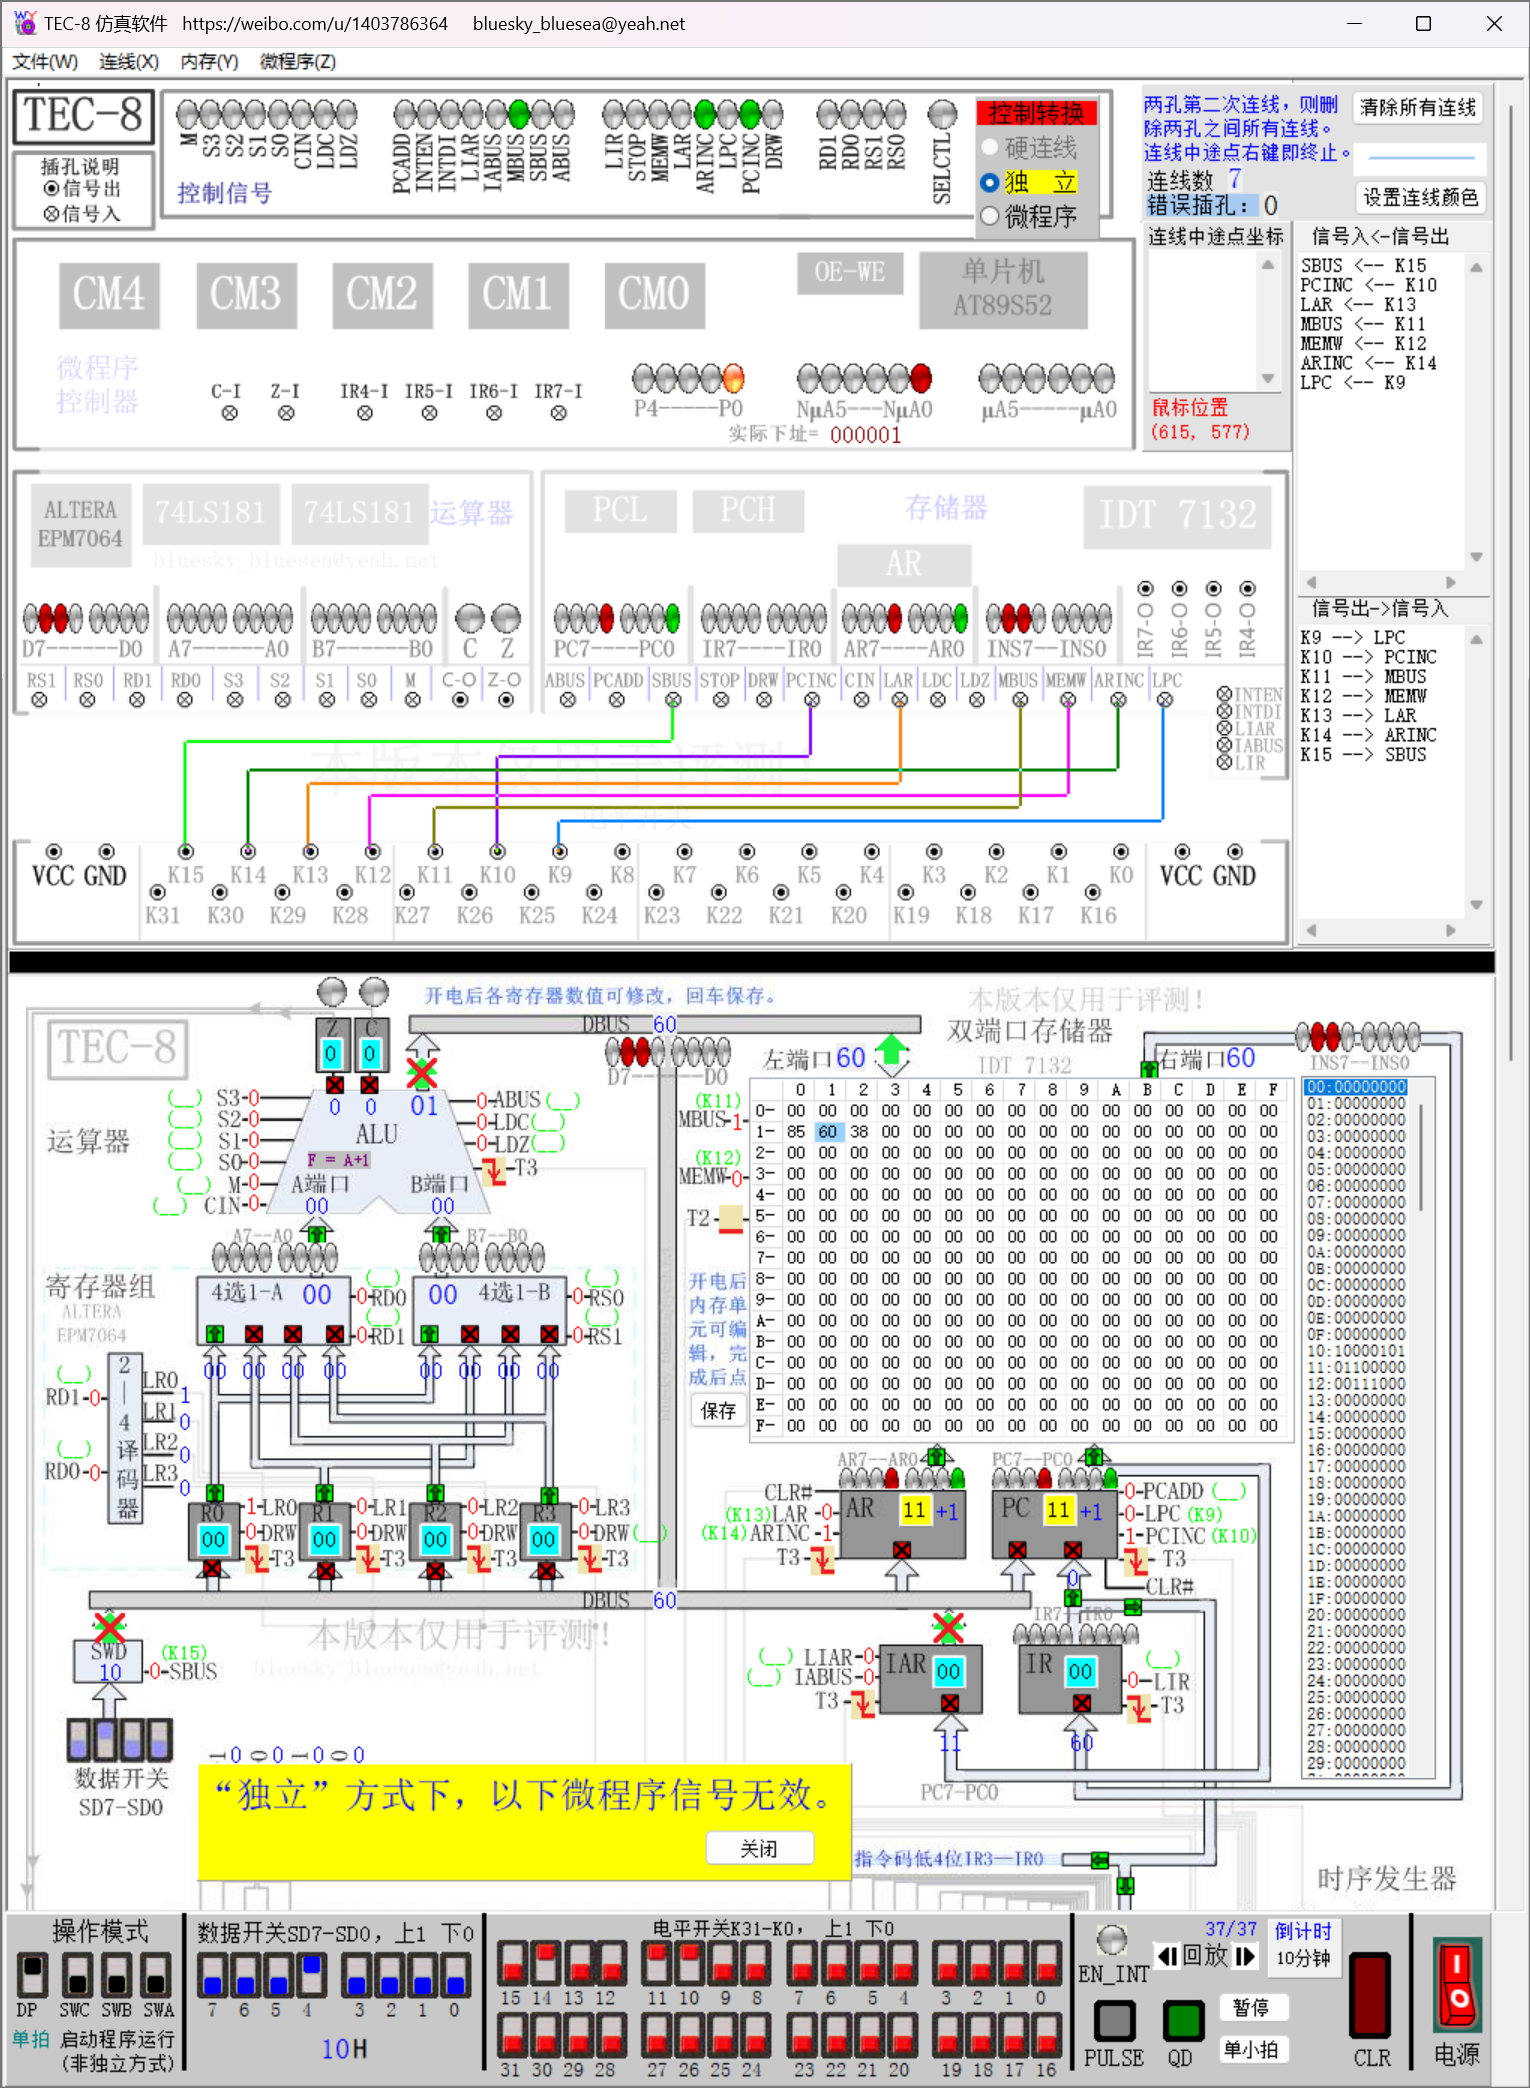
\includegraphics[width=0.3\textwidth]{screenshots/2.2.8.png}
              }
              \subfigure[读取内存12H]{
                  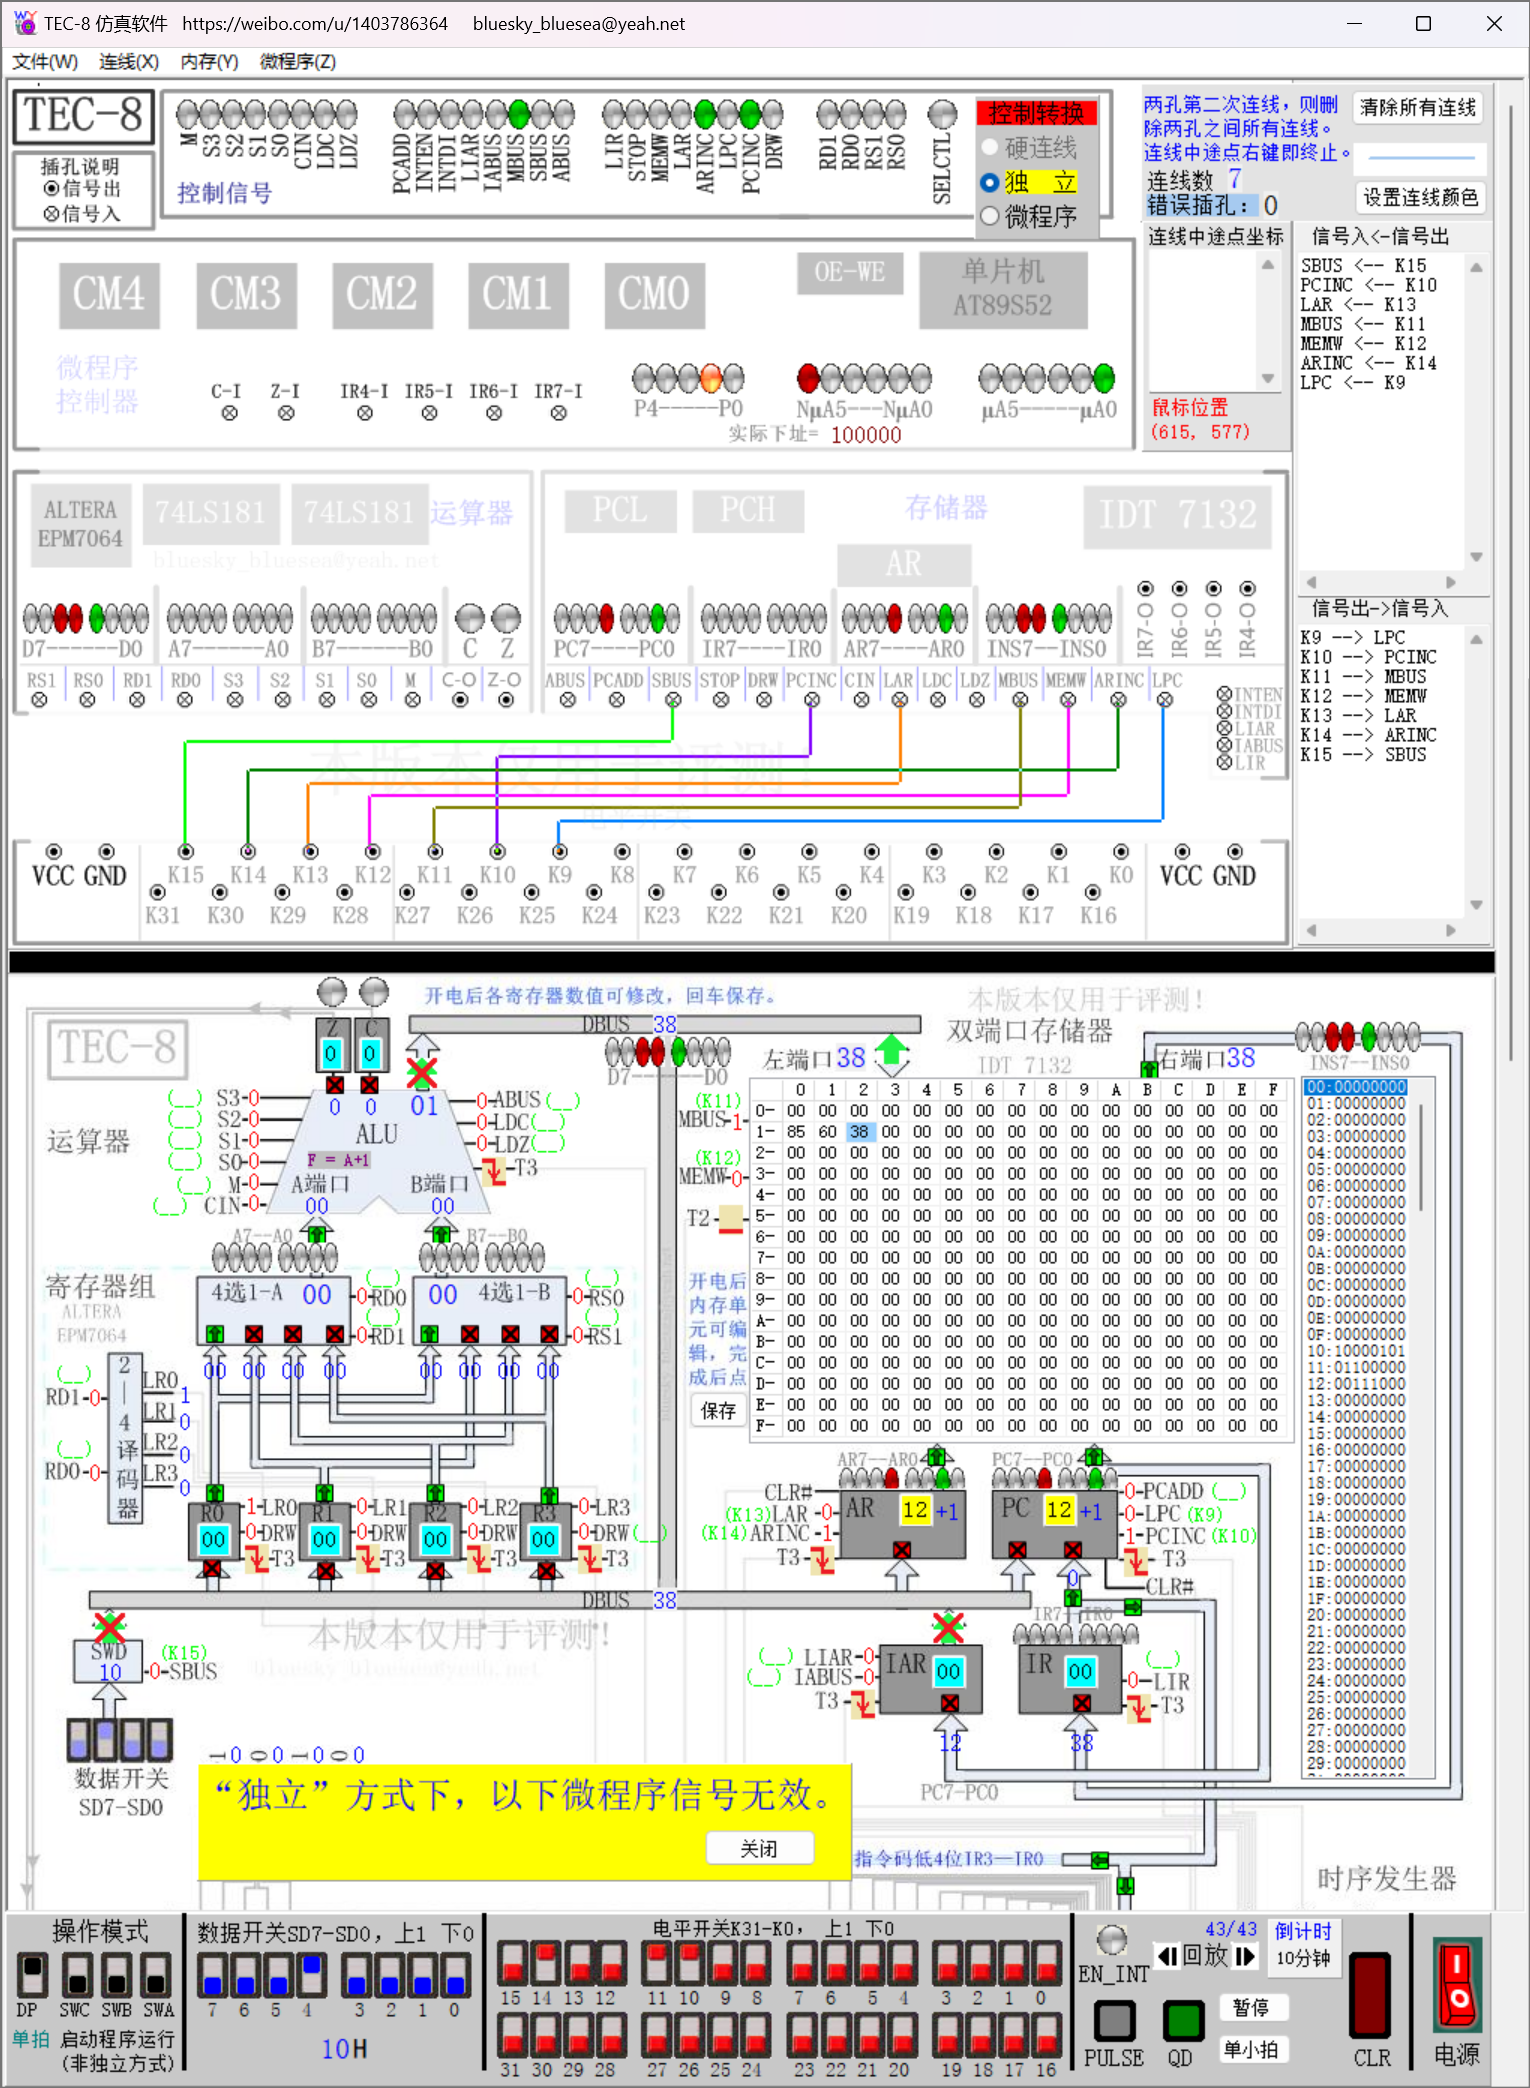
\includegraphics[width=0.3\textwidth]{screenshots/2.2.9.png}
              }
              \caption{数据操作 (独立)}
              \label{fig:2.3}
          \end{figure}

\end{enumerate}

\section{思考与心得}

\subsection{思考}

\subsubsection{实验中各个信号的作用}

\begin{itemize}

    \item SBUS, MBUS

          分别控制数据开关和双端口存储器对DBUS总线的写入. 在输入地址和数据时需要开启SBUS开关, 从存储器左端口读出数据时需要开启MBUS开关, 其余时候不需要开启这两个开关. 这两个开关也不能同时开启, 否则会对总线的写入造成冲突.

    \item LPC, LAR

          分别控制PC和AR是否从DBUS总线读入数据. 在设置初始地址和地址复位时需要开启, 其他时候不开启.

    \item PCINC, ARINC

          分别控制PC和AR是否自增. 设置完初始地址后在写入和读取数据时需要开启.

    \item MEMW

          控制存储器是否将DBUS总线上的数据读入内存. 在写入数据时需要开启.

\end{itemize}

\subsubsection{在通过左端口向双端口 RAM 写数时, 在右端口可以同时观测到左端口写入的数吗? 为什么?}

可以. 因为根据题目的设置, PC地址与AR地址是同步的, 向同一个地址写入数据后右端口就能立即读出该数据.

\subsection{心得}

通过这次实验, 我对计算器中存储器, PC寄存器, AR寄存器以及数据总线等部件都有了更深入的了解. 我也对双端口存储器的工作方式有了一定的了解.

\end{document}